\documentclass[11pt,a4paper]{article}

% ============================================================
% PACKAGES
% ============================================================
\usepackage[utf8]{inputenc}
\usepackage[T1]{fontenc}
\usepackage{amsmath}
\usepackage{amssymb}
\usepackage{graphicx}
\usepackage{float}
\usepackage{booktabs}
\usepackage{multirow}
\usepackage[margin=2.5cm]{geometry}
\usepackage{listings}
\usepackage{xcolor}
\usepackage{caption}
\usepackage{subcaption}
\usepackage[hidelinks]{hyperref}
\usepackage{titlesec}
\usepackage{tikz}
\usetikzlibrary{arrows.meta,positioning,shapes.geometric}

% ============================================================
% CODE LISTING STYLE
% ============================================================
\definecolor{codegray}{gray}{0.9}
\definecolor{codegreen}{rgb}{0,0.5,0}
\definecolor{codeblue}{rgb}{0,0,0.6}
\lstset{
    backgroundcolor=\color{codegray},
    basicstyle=\ttfamily\footnotesize,
    frame=single,
    breaklines=true,
    captionpos=b,
    tabsize=4,
    numbers=left,
    numberstyle=\tiny\color{gray},
    keywordstyle=\color{codeblue},
    commentstyle=\color{gray},
    stringstyle=\color{codegreen},
    showstringspaces=false
}

% ============================================================
% CUSTOM COMMANDS
% ============================================================
\newcommand{\Freq}{\ensuremath{F}}
\newcommand{\Key}[1]{\texttt{#1}}

\titleformat{\section}{\Large\bfseries}{\thesection.}{0.6em}{}
\titleformat{\subsection}{\large\bfseries}{\thesubsection.}{0.6em}{}

% Every top-level section (and the bibliography) starts on a fresh page.
\newcommand{\sectionbreak}{\clearpage}

% ============================================================
% DOCUMENT
% ============================================================
\title{
    \vspace{-2em}
    \textbf{Acoustic Side-Channel Attack on Mechanical Keyboards}\\[0.5em]
    \large Software-Based Keystroke Reconstruction Using Frequency Signatures
    \vspace{-0.5em}
}
\author{%
    \normalsize Cyber-Physical Systems Project\\[0.4em]
    \textbf{By} \\[0.3em]
    \begin{tabular}{ll}
        23MEI10066 & Dev Soni \\
        23MEI10067 & Shreyansh Tripathi \\
        23MEI10069 & Himalaya Yadav \\
        23MEI10070 & Eklavya Mathur \\
        23MEI10085 & Akshit Agrawal \\
    \end{tabular}\\[1cm]
    \textbf{Course Instructor} \\[0.3em]
    Dr. Hemraj S Lamkuche \\
    School of Computing Science Engineering and Artificial Intelligence \\
    VIT Bhopal University, Sehore \\
    Madhya Pradesh
}
\date{\today}

\begin{document}

\maketitle
\thispagestyle{empty}

\begin{center}
    \rule{\textwidth}{0.4pt}
\end{center}

\clearpage
\tableofcontents
\listoffigures
\listoftables
\clearpage

% ============================================================
% 1. TEAM ROLES AND CONTRIBUTIONS
% ============================================================
\section{Team Roles and Contributions}
\label{sec:roles}

This project was carried out by a five-member team. The work was partitioned so
that two members carried the core of the system and the remaining three each
owned a well-defined supporting component. \textbf{Eklavya Mathur} was
responsible for the real-time reconstruction engine and the formal
Cyber-Physical Systems (CPS) verification layer. \textbf{Himalaya Yadav} was
responsible for the frequency-signature model, the waveform and spectrogram
visualization, and the security analysis. \textbf{Dev Soni} implemented the
graphical user interface, \textbf{Shreyansh Tripathi} built the automated test
suite, and \textbf{Akshit Agrawal} implemented the on-screen keypad and
punctuation support and maintained the project documentation. The majority of
the design, implementation, and analysis effort---the core engine, the CPS
verification, the signal model, the visualization, and the security
analysis---was carried jointly by Eklavya Mathur and Himalaya Yadav; the GUI,
the test suite, and the keypad, punctuation, and documentation work were divided
among the other three members. All five members took part in the design
discussions, code reviews, and the proofreading of this report.

\begin{table}[H]
    \centering
    \begin{tabular}{@{}p{3.2cm}p{3.3cm}p{8.0cm}@{}}
        \toprule
        \textbf{Member (ID)} & \textbf{Primary role} &
        \textbf{Principal contributions} \\
        \midrule
        Eklavya Mathur\newline (23MEI10070) &
        \emph{Lead} --- real-time engine and CPS verification &
        Overall system architecture; core reconstruction pipeline
        (\texttt{identify\_key} ranking function, \texttt{process\_frequency},
        \texttt{reconstruct\_sequence}); robust multi-trial WCET
        (median + P95) measurement and deadline checking;
        \texttt{check\_invariants}, \texttt{liveness\_test},
        \texttt{termination\_test}; deterministic separation proof, complexity
        analysis, and the ranking/variant-function termination argument;
        optimization flow; integration and authoring of this report. \\
        \midrule
        Himalaya Yadav\newline (23MEI10069) &
        \emph{Lead} --- signal model, visualization, and security &
        Design of the 48-key \texttt{KEY\_FREQUENCIES} table on the 30~Hz grid;
        \texttt{generate\_frequency} and the $\pm 5$~Hz bounded-noise model;
        \texttt{waveform\_visualization.py} (numpy-vectorised sine synthesis,
        sliding Hann-windowed FFT spectrogram, incremental live updaters);
        \texttt{make\_figures.py} deterministic figure generator; threat model,
        mitigation survey, and the related-work comparison. \\
        \midrule
        Dev Soni\newline (23MEI10066) &
        \emph{Support} --- graphical user interface &
        \texttt{AcousticSideChannelApp} tkinter shell; multi-line paragraph
        input box; Analysis and Waveform tabs; wiring of keypad events to the
        live plots; the display path of the single-source
        \texttt{format\_report()}. \\
        \midrule
        Shreyansh Tripathi\newline (23MEI10067) &
        \emph{Support} --- automated test suite &
        \texttt{tests/test\_frequency.py} (62 tests): invariant, ranking,
        pipeline, sequence, and multi-line paragraph reconstruction tests, plus
        headless GUI-helper tests using a stubbed application object; the
        requirement-to-test traceability matrix. \\
        \midrule
        Akshit Agrawal\newline (23MEI10085) &
        \emph{Support} --- keypad, punctuation, and documentation &
        On-screen keypad with append-at-\texttt{END} behaviour; the 11
        punctuation signatures and their tests; widening of the spectrogram
        band to 1900~Hz; \texttt{README}, \texttt{requirements.txt}, and the
        \texttt{docs/} guides; formatting and proofreading of this report. \\
        \bottomrule
    \end{tabular}
    \caption{Division of work among the team members.}
    \label{tab:roles}
\end{table}

% ============================================================
% 2. UNDERSTANDING THE PROJECT
% ============================================================
\section{Understanding the Project}
\label{sec:understanding}

This section introduces the project, identifies the system aspect it targets,
defines the key technical terms used throughout the report, states the problem
in a concise form, and lays out the structure of the rest of the document.

\subsection{Targeted System Aspect}

A cyber-physical system can be evaluated along several orthogonal quality
attributes. This project deliberately targets specific aspects of the design
and exposes the trade-offs involved. The following table summarises how each
attribute is (or is not) addressed by the simulator.

\begin{table}[H]
    \centering
    \begin{tabular}{@{}llp{9cm}@{}}
        \toprule
        \textbf{Aspect} & \textbf{Role} & \textbf{How it is addressed} \\
        \midrule
        Design & Active & Modular separation of core logic, GUI, and
            visualization; single-source \texttt{format\_report()} so the GUI
            output and exported file are identical. \\
        Performance & Active & Real-time deadline of 50 ms; robust multi-trial
            WCET (median + P95) measurement; numpy-vectorised signal
            generation. \\
        Security & Active & Frequency-signature confidentiality; the
            \Key{UNKNOWN} safety state prevents incorrect key assignment;
            threat modelling against real acoustic side-channel eavesdroppers.
            \\
        Reliability & Active & Invariant checking, deterministic constant
            table, and 62 unit tests guarding reconstruction correctness. \\
        Scalability & Passive & The 48-key constant table is $O(1)$ lookup;
            \texttt{MAX\_PLOT\_KEYS} bounds rendering so paragraph-length input
            remains responsive, but large-key-set growth is not the focus.
            \\
        \bottomrule
    \end{tabular}
    \caption{System aspects targeted by the project.}
    \label{tab:aspects}
\end{table}

\noindent
The simulator is chiefly a \emph{performance} and \emph{security} exercise: it
must reconstruct keystrokes within a hard real-time deadline while never
emitting an incorrect key. Reliability and extensibility support these goals,
while scalability is deliberately constrained to keep the model tractable.

\subsection{Key Technical Terms}

The following glossary defines the central terms used in this report in a
single line each.

\begin{table}[H]
    \centering
    \begin{tabular}{@{}p{4.5cm}p{11cm}@{}}
        \toprule
        \textbf{Term} & \textbf{Definition} \\
        \midrule
        Acoustic side-channel attack & Extraction of secret information (here,
            keystrokes) by observing unintended physical emanations---the sound
            of key presses. \\
        Frequency signature & The unique, predefined frequency (in Hz) assigned
            to each key so it can be told apart from every other key. \\
        WCET & \emph{Worst-Case Execution Time}: the longest time a real-time
            task may take to complete. \\
        Deadline & The time bound ($50$ ms here) within which the task must
            finish to satisfy the real-time requirement. \\
        Tolerance & The maximum accepted frequency error ($8$ Hz) for a match to
            be considered valid. \\
        Confidence & A score $C \in [0,1]$ expressing how close a detected
            frequency is to a key's signature: $C = 1 - V/\text{tolerance}$. \\
        Invariant & A property that must hold true at every point of program
            execution. \\
        Liveness & The property that the system is always able to eventually
            produce an output for new input. \\
        Termination & The property that any finite input sequence finishes in
            bounded time. \\
        Spectrogram & A frequency-versus-time heatmap showing how signal energy
            is distributed across frequencies. \\
        FFT & \emph{Fast Fourier Transform}: an algorithm to convert a
            time-domain signal into its frequency components. \\
        UNKNOWN & A safe fallback state returned when no key matches within
            tolerance, preventing incorrect classification. \\
        Ranking function & The error metric $V = |F_d - F_e|$ (absolute
            difference between detected and expected frequency) that the
            matcher minimises and that also serves as a variant function for
            termination. \\
        \bottomrule
    \end{tabular}
    \caption{Key technical terms used in the report.}
    \label{tab:glossary}
\end{table}

\subsection{Problem Statement}

This project implements a \emph{software-based simulation} of an acoustic
side-channel attack on a mechanical keyboard: it assigns each of 48 keys a
unique frequency signature, simulates the frequency that would be observed for
a key press, and reconstructs the typed keystroke sequence by matching the
observed frequency back to a key within a tolerance, all within a 50 ms
real-time deadline.

\noindent
The problem it solves is demonstrating, entirely in software, that keystroke
reconstruction is feasible from frequency signatures alone and that the
resulting system satisfies the formal Cyber-Physical Systems (CPS) verification
requirements (deadline, invariants, liveness, termination, ranking/error
function, and safety). The main hardware resource used is an ordinary
general-purpose computer (a laptop or desktop) running Python; no microphone,
no dedicated sensing hardware, and no embedded controller are required.

\paragraph{What this project is, and is not.}
Because the simulation framing is central to honest claims, it is useful to make
the boundary explicit.

\begin{table}[H]
    \centering
    \begin{tabular}{@{}p{7cm}p{7cm}@{}}
        \toprule
        \textbf{This project IS} &
        \textbf{This project is NOT} \\
        \midrule
        A software simulation of keystroke reconstruction from frequency
        signatures. &
        A real attack on real keyboards or microphones. \\
        A demonstration of the acoustic side-channel \emph{concept}. &
        A capture of real acoustic emanations. \\
        A formal CPS verification case study
        (deadline, WCET, invariants, liveness, termination). &
        A production-grade security tool. \\
        An interactive GUI demo with waveform and spectrogram visualization. &
        A hardware/embedded implementation (though its data structures
        would port to one). \\
        \bottomrule
    \end{tabular}
    \caption{Explicit boundary between the simulation and the real-world attack
             it illustrates.}
    \label{tab:isnot}
\end{table}

\subsection{Structure of This Report}

The remainder of the report follows the project brief. Sections~\ref{sec:principle}
to~\ref{sec:conclusion} together form the \emph{technical context} of the
project: Section~\ref{sec:principle} states the underlying principle (why the
approach works, not just what it is), Section~\ref{sec:whycps} explains why it
matters for embedded and cyber-physical systems, Section~\ref{sec:impl}
describes the implementation (architecture, flowchart, hardware, and software
design), Section~\ref{sec:results} presents the testing methodology and results
as tables and figures, Section~\ref{sec:analysis} gives the analysis and
evaluation (theory, statistics, an aspect-by-aspect assessment, problems, bugs,
optimization, and limitations), and Section~\ref{sec:conclusion} concludes. A
short bibliography follows.

% ============================================================
% 3. UNDERLYING PRINCIPLE
% ============================================================
\section{Underlying Principle}
\label{sec:principle}

This section explains \emph{why} the approach works: why a frequency signature
can identify a key, how the idea relates to the published literature on acoustic
side channels, and how the physical idea is distilled into a tractable model
with a provable separation margin.

\subsection{Why a Frequency Signature Can Identify a Key}

The central idea is that every key on a keyboard has a characteristic acoustic
signature. In a real physical system, pressing different keys produces slightly
different sounds because the key strikes a different point, travels a different
distance, and resonates through the keyboard chassis differently. These
differences manifest as measurable differences in the frequency content of the
sound.

\subsection{Related Work: Acoustic Side-Channel Attacks}
\label{sec:related-bg}

The concept of extracting keystrokes from acoustic emanations is not new.
Asonov and Agrawal (2004) were among the first to demonstrate \emph{keyboard
acoustic emanations} as a viable side channel, using frequency-feature
classification. More recent work has two broad branches. The first performs
\emph{frequency-domain analysis}: it converts recordings into the frequency
domain with the Fast Fourier Transform (FFT) or Mel-frequency cepstral
coefficients (MFCCs) and classifies each keystroke. The second applies
\emph{deep learning}: modern systems such as the CoAtNet model of Harrison et
al.\ (2023) classify keystrokes from mel-spectrograms, achieving accuracy of
$95\%$ when trained on keystrokes recorded by a smartphone and $93\%$ when
trained on audio compressed through the Zoom video-conferencing codec. Public
toolkits such as Gerganov's \texttt{kbd-audio} (``KeyTap'') reconstruct
keystrokes in real time by matching recorded audio against per-key
\emph{fingerprints} learned from a known transcript. A quantitative comparison
of this project with these works is given in Section~\ref{sec:related}.

These works establish two important facts for this project's context:

\begin{itemize}
    \item Real keystroke acoustics are \emph{broadband, transient} signals:
          a key press is a short burst of sound spread across many
          frequencies. Distinguishing keys therefore requires either rich
          spectral features (FFT/MFCC/spectrograms) or learned patterns, not a
          single pure tone.
    \item Despite this complexity, the \emph{principle} behind the attack is
          simple and robust: different keys produce measurably different
          sounds, and a classifier (whether geometric frequency matching or a
          deep network) can map those sounds back to keys.
\end{itemize}

This project deliberately compresses the first fact and keeps the second. It
replaces real broadband recordings with clean, well-separated per-key
frequencies so that classification reduces to unambiguous nearest-frequency
matching. The result is a faithful demonstration of the \emph{concept} and of
the CPS verification layer, without pretending to model real signal physics.

\subsection{From Physical Idea to Model}

This project distils the physical idea into a clean, tractable model. Rather
than deriving frequencies from real recordings, each key is assigned a
predefined, \emph{unique} frequency following a regular pattern:

\[
F(\text{key}_i) = 440 + 30 \cdot (i - 1) \quad \text{Hz},
\]

for $i$ counting keys in order from \Key{A} (440 Hz) upward through the 26
letters, SPACE, the 10 digits, and 11 punctuation marks, ending at 1850 Hz.
This provides a total of 48 distinct signatures.

Why does this work? The matching procedure relies on three quantities being
chosen so that keys are \emph{well separated} relative to the measurement
noise:

\begin{enumerate}
    \item \textbf{Uniqueness:} no two keys share a frequency, so a frequency
          can be mapped back to exactly one key.
    \item \textbf{Separation:} adjacent keys are 30 Hz apart, which is much
          larger than the $\pm 5$ Hz synthetic noise and comfortably larger
          than the 8 Hz tolerance.
    \item \textbf{Tolerance-bound guarantee:} the maximum synthetic noise
          ($\pm 5$ Hz) is strictly less than half the spacing (15 Hz) and less
          than the tolerance (8 Hz), so a correct key always remains inside
          its own detection band even in the worst case.
\end{enumerate}

If the noise were larger than half the spacing, or if two keys shared a
frequency, the reconstruction would become ambiguous. The separation margin is
therefore the root cause of the system's correctness: it is this margin, not
any particular frequency value, that makes identification reliable.

\subsection{The Matching Rule}

Given a detected frequency $F_{\text{detected}}$, the matcher computes an error
for every candidate key:

\[
V_i = |F_{\text{detected}} - F_{\text{expected},i}|.
\]

The key with the smallest error is chosen, but only if that smallest error is
within the tolerance:

\[
\min_i V_i \le \text{TOLERANCE} \;\Rightarrow\; \text{key} = \arg\min_i V_i,
\qquad\text{otherwise key} = \Key{UNKNOWN}.
\]

The \Key{UNKNOWN} result is a deliberate safety measure: the software never
forces an incorrect key when no signature is close enough. This is the single
most important design principle for the security aspect of the system.

% ============================================================
% 4. RELEVANCE TO EMBEDDED AND CYBER-PHYSICAL SYSTEMS
% ============================================================
\section{Relevance to Embedded and Cyber-Physical Systems}
\label{sec:whycps}

The simulator is a faithful model of the constraints that real embedded and CPS
applications must respect. Although it runs on a general-purpose computer, it
demonstrates the same fundamental requirements that appear in any real-time,
resource-constrained, safety-critical system.

\subsection{Real-Time and Performance Constraints}

A keystroke is an event that must be processed before the next one arrives or
before the reconstruction becomes out of order. This is a classic real-time
task. The project imposes a deadline:

\[
T_{\text{WCET}} < T_{\text{deadline}} = 50 \text{ ms}.
\]

The total processing time for a key is the sum of the individual stages:

\[
T_{\text{total}} = T_{\text{input}} + T_{\text{frequency}}
+ T_{\text{analysis}} + T_{\text{matching}} + T_{\text{output}}.
\]

Because a single timing measurement is noisy, the system measures the
reconstruction over multiple trials and reports robust statistics---the
\emph{median} (typical worst case) and the \emph{P95} (conservative worst
case)---so the reported WCET is not distorted by scheduler or measurement
noise. This mirrors how a real embedded engineer would characterise a task on
an embedded target: measure repeatedly, report a robust worst case, and prove
it fits the deadline.

\paragraph{Performance characterisation.}
Each keystroke involves a bounded number of operations: a dictionary lookup to
generate the frequency and a single pass over the 48-entry constant table to
perform nearest-match classification. Per-key work is therefore $O(1)$ with
respect to everything except the fixed 48-entry scan, and processing a whole
text of $n$ keys is $O(n)$. There is no sorting of the input, no search over a
growing collection, and no unbounded allocation per key. The measured per-key
time is in the tens of microseconds, orders of magnitude below the deadline.
This analysis is expanded with figures in Section~\ref{sec:results}.

\subsection{Storage Constraints}

The entire ``knowledge'' of the system is a constant table of 48
(key, frequency) pairs. This maps to a static lookup table in a real embedded
system---an extremely compact data structure. The memory footprint is
independent of the input length, and a lookup is $O(1)$.

Stored as a Python dict, the table occupies on the order of a few kilobytes.
Projected onto an embedded target, the (key, frequency) pairs fit in a few
hundred bytes of read-only memory (roughly 200 bytes of flash/ROM plus the
code), so a resource-constrained device could hold the entire signature
database on-chip. Runtime memory is proportional only to the length of the
current input, and every per-key operation uses a fixed, constant amount of
scratch space.

\subsection{Reliability and Safety Constraints}

Real CPS applications must never exhibit unsafe behaviour. Here the safety
requirement is that the system must never:

\begin{itemize}
    \item accept an invalid frequency as a valid key,
    \item allow two keys to share a frequency,
    \item emit an incorrect key mapping, or
    \item exceed the deadline and lose input.
\end{itemize}

These are captured as formal invariants and enforced by a dedicated check
and by the \Key{UNKNOWN} fallback, exactly as a safety monitor would be
implemented in a real embedded controller.

\subsection{CPS Concepts Mapped to Implementation}

\begin{table}[H]
    \centering
    \begin{tabular}{@{}lp{10.5cm}@{}}
        \toprule
        \textbf{CPS concept} & \textbf{How the simulator realises it} \\
        \midrule
        Real-time task & \texttt{process\_frequency}: analyse + match + identify. \\
        WCET & \texttt{reconstruct\_sequence\_wcet} $\rightarrow$ median + P95
            over \texttt{WCET\_TRIALS} $=20$ trials. \\
        Deadline & \texttt{DEADLINE\_MS} $=50$ ms, pass/fail checked. \\
        Invariants & \texttt{check\_invariants}: positive, unique, valid. \\
        Liveness & \texttt{liveness\_test}: new input always yields output. \\
        Termination & \texttt{termination\_test}: finite input finishes. \\
        Ranking function & \texttt{identify\_key}: $V=|F_d-F_e|$ minimised. \\
        Confidence & \texttt{compute\_confidence}: $C = 1 - V/\text{tol}$. \\
        Safety & \texttt{UNKNOWN} state when out of tolerance. \\
        \bottomrule
    \end{tabular}
    \caption{Mapping CPS verification concepts to their implementation.}
    \label{tab:cpsmap}
\end{table}

% ============================================================
% 5. IMPLEMENTATION
% ============================================================
\section{Implementation}
\label{sec:impl}

This section describes the physical resources, the overall architecture, the
control flow of the core task, the ranking/variant function that guarantees
termination, and the software design of the simulator.

\subsection{System Architecture}

The system follows a layered architecture: a tkinter GUI front-end delegates
to a pure core-logic module, which in turn delegates plotting to a separate
visualization module. Keeping the core logic independent of the GUI makes it
headless-testable.

\begin{figure}[H]
    \centering
    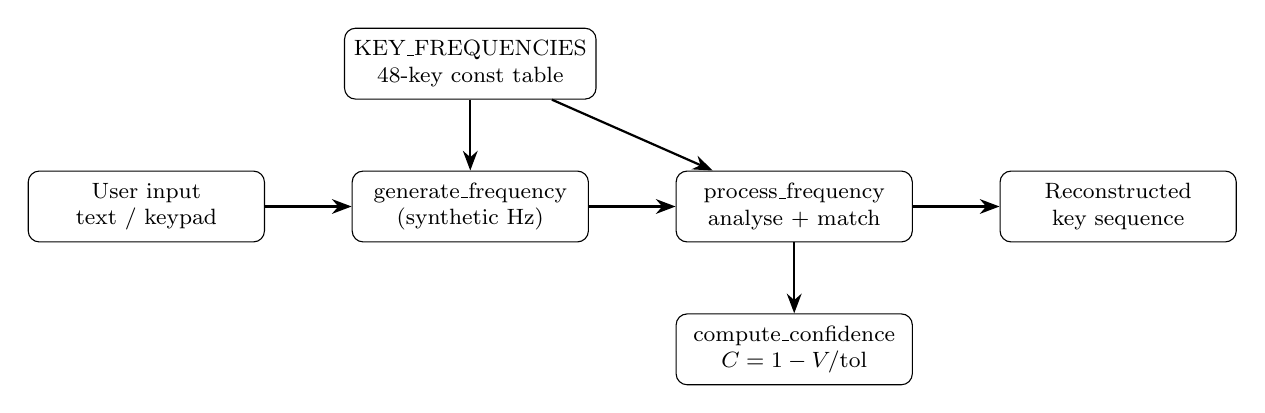
\begin{tikzpicture}[
        node distance=0.9cm and 1.1cm,
        box/.style={rectangle, draw, rounded corners, minimum width=3.0cm,
                    minimum height=0.9cm, align=center, font=\footnotesize},
        arrow/.style={-{Stealth[length=2.5mm]}, thick}
    ]
        \node[box] (in) {User input\\ text / keypad};
        \node[box, right=of in] (freq) {generate\_frequency\\ (synthetic Hz)};
        \node[box, right=of freq] (proc) {process\_frequency\\ analyse + match};
        \node[box, right=of proc] (out) {Reconstructed\\ key sequence};
        \node[box, below=of proc] (conf) {compute\_confidence\\ $C = 1 - V/\text{tol}$};
        \node[box, above=of freq] (data) {KEY\_FREQUENCIES\\ 48-key const table};

        \draw[arrow] (in) -- (freq);
        \draw[arrow] (freq) -- (proc);
        \draw[arrow] (proc) -- (out);
        \draw[arrow] (proc) -- (conf);
        \draw[arrow] (data) -- (freq);
        \draw[arrow] (data) -- (proc);
    \end{tikzpicture}
    \caption{High-level system architecture: a labelled block diagram of the
             data flow from user input to reconstructed keystrokes.}
    \label{fig:arch}
\end{figure}

The block diagram in Figure~\ref{fig:arch} shows how the request flows. User
input is converted to a list of key symbols, each key is mapped to its
predefined frequency, the frequency is analysed and matched against the
constant table, and the result is a reconstructed sequence with a per-key
confidence value.

\subsection{Control-Flow Flowchart of the Core Pipeline}

Figure~\ref{fig:flowchart} is the control-flow flowchart of the reconstruction
task: the outer loop of \texttt{reconstruct\_sequence} driving
\texttt{identify\_key} for each character. It makes the two decision points
explicit---whether a character maps to a key at all, and whether the best match
lies within tolerance---and shows the \Key{UNKNOWN} safety branch.

\begin{figure}[H]
    \centering
    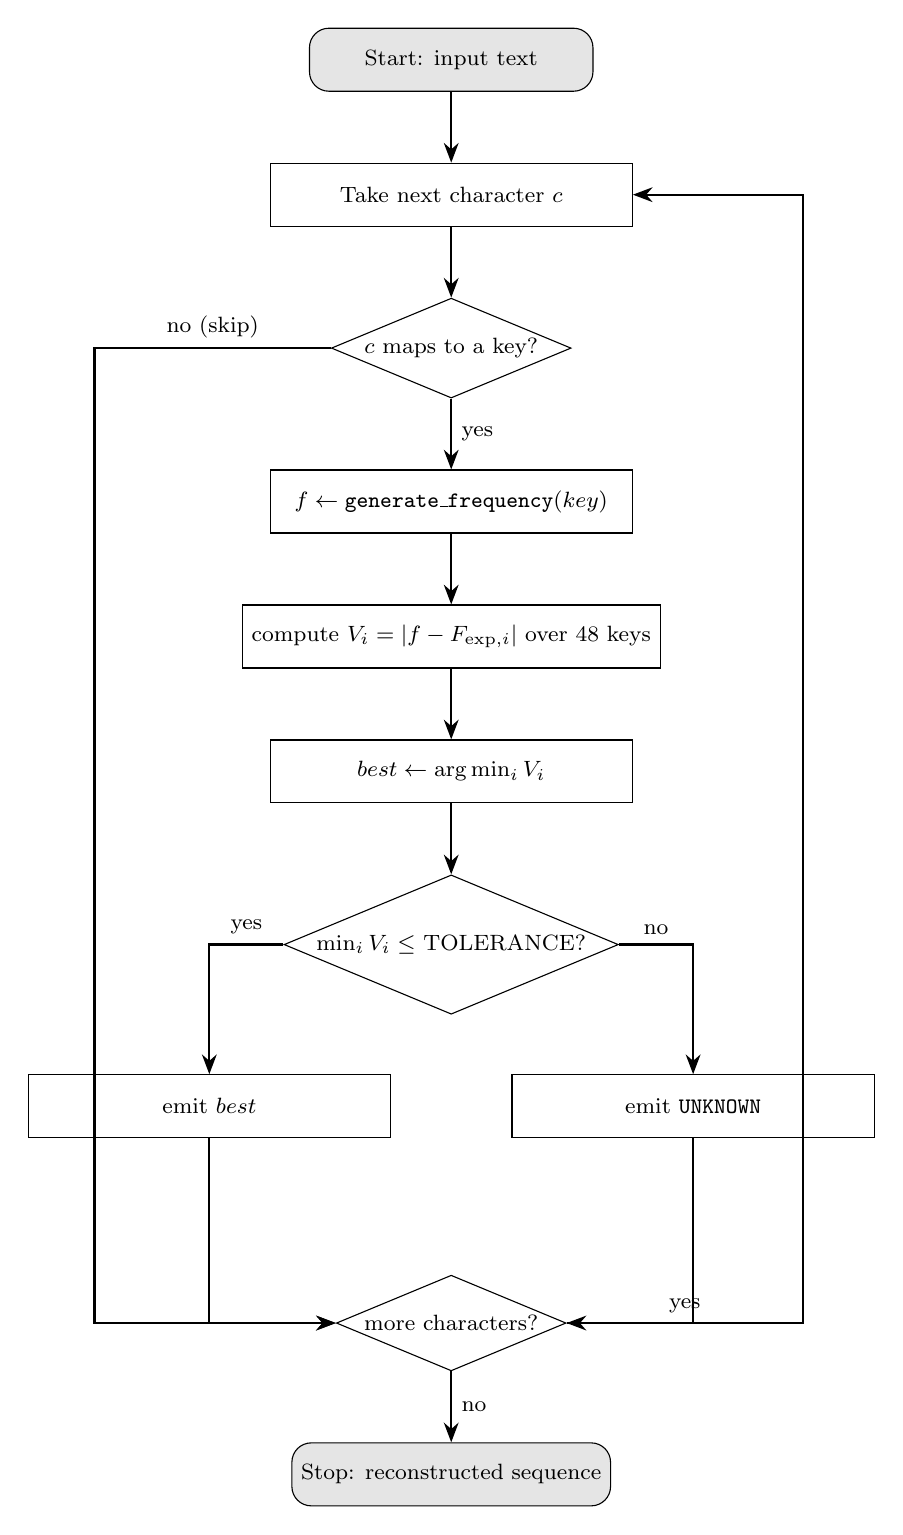
\begin{tikzpicture}[
        node distance=0.9cm,
        font=\footnotesize,
        term/.style={rectangle, rounded corners=7pt, draw, fill=codegray,
                     minimum width=3.6cm, minimum height=0.8cm, align=center},
        proc/.style={rectangle, draw, minimum width=4.6cm, minimum height=0.8cm,
                     align=center},
        dec/.style={diamond, draw, aspect=2.4, inner sep=1pt, align=center},
        a/.style={-{Stealth[length=2.5mm]}, thick}
    ]
        \node[term] (start) {Start: input text};
        \node[proc, below=of start] (next) {Take next character $c$};
        \node[dec, below=of next] (map) {$c$ maps to a key?};
        \node[proc, below=of map] (gen) {$f \gets \texttt{generate\_frequency}(key)$};
        \node[proc, below=of gen] (scan) {compute $V_i = |f - F_{\text{exp},i}|$ over 48 keys};
        \node[proc, below=of scan] (best) {$best \gets \arg\min_i V_i$};
        \node[dec, below=of best] (tol) {$\min_i V_i \le$ TOLERANCE?};
        \node[proc, below left=1.2cm and -0.3cm of tol] (emit) {emit $best$};
        \node[proc, below right=1.2cm and -0.3cm of tol] (unk) {emit \texttt{UNKNOWN}};
        \node[dec, below=3.3cm of tol] (more) {more characters?};
        \node[term, below=of more] (stop) {Stop: reconstructed sequence};

        \draw[a] (start) -- (next);
        \draw[a] (next) -- (map);
        \draw[a] (map) -- node[right]{yes} (gen);
        \draw[a] (gen) -- (scan);
        \draw[a] (scan) -- (best);
        \draw[a] (best) -- (tol);
        \draw[a] (tol) -| node[near start, above]{yes} (emit);
        \draw[a] (tol) -| node[near start, above]{no} (unk);
        \draw[a] (emit) |- (more);
        \draw[a] (unk) |- (more);
        \draw[a] (more) -- node[right]{no} (stop);
        \draw[a] (map.west) -- ++(-3.0,0) node[midway, above]{no (skip)} |- (more.west);
        \draw[a] (more.east) -- ++(3.0,0) node[midway, above]{yes} |- (next.east);
    \end{tikzpicture}
    \caption{Control-flow flowchart of the reconstruction pipeline. Unmapped
             characters are skipped; the \Key{UNKNOWN} branch is the safety
             fallback taken when no signature lies within tolerance.}
    \label{fig:flowchart}
\end{figure}

\subsection{Ranking / Variant Function and Termination}
\label{sec:variant}

The reconstruction contains two bounded loops, and each is governed by a
non-negative \emph{variant} (ranking) function that strictly decreases. This is
a Lyapunov-style argument for termination: a quantity bounded below by zero that
decreases on every step must reach its bound in finitely many steps.

\paragraph{Inner loop (\texttt{identify\_key}).}
The loop iterates over the fixed 48-entry table. Let the variant be the number
of unexamined keys, $n_{\text{rem}} \in \{48, 47, \ldots, 0\}$. Each iteration
decrements $n_{\text{rem}}$ by exactly one, and it is bounded below by $0$, so
the loop terminates after exactly 48 steps. The quantity the loop
\emph{minimises}, $V = |F_d - F_e|$, is itself non-negative and bounded above by
the span of the table ($\approx 1410$ Hz), and the running best error
\texttt{best\_error} is monotonically non-increasing---a second ranking function
confirming progress toward the nearest signature.

\paragraph{Outer loop (\texttt{reconstruct\_sequence}).}
For an input of $n$ characters, let the variant be the count of unprocessed
characters. It starts at $n$, strictly decreases by one on every iteration
(whether the character is mapped and emitted, or skipped), and is bounded below
by $0$. Hence any finite input terminates in at most $n$ iterations.

\paragraph{Combined bound.}
Total work is bounded by $48 \cdot n$ absolute-difference operations, so
$T_{\text{total}}$ is finite for every finite input and, as
Section~\ref{sec:analysis} shows, far below the 50 ms deadline. The function
\texttt{termination\_test()} exercises this directly with a 1000-character
input.

\subsection{Hardware and Platform Details}

Because this is a software simulation, the hardware requirements are minimal
and no dedicated controller or sensing hardware is used.

\begin{itemize}
    \item \textbf{Host platform:} any general-purpose laptop or desktop
          computer (x86-64 or ARM). The project is developed and tested on a
          Linux host.
    \item \textbf{Controller:} none---there is no microcontroller, no FPGA, no
          embedded board. The ``controller'' is the host CPU running the Python
          interpreter.
    \item \textbf{Microphone / audio:} none. All frequencies are predefined
          constants; no real acoustic signal is captured.
    \item \textbf{Display:} a graphical display is needed only to run the
          tkinter GUI; the core logic and tests run headlessly.
    \item \textbf{Software runtime:} Python 3.11+ with the standard library,
          numpy, matplotlib, tkinter, and pytest.
\end{itemize}

The absence of a physical keyboard and microphone is intentional and central to
the project's framing: it is a \emph{simulation} of the side-channel concept
and its CPS verification, not a functional attack on real hardware.

\subsection{Software Design}

The software is organised into two source files.

\begin{itemize}
    \item \texttt{src/acoustic\_side\_channel.py}---core logic and GUI:
          the frequency database, invariant checker, frequency generator,
          matcher, confidence, WCET measurement, \texttt{liveness}/
         \texttt{termination} tests,
          report builder, and the tkinter application.
    \item \texttt{src/waveform\_visualization.py}---the matplotlib/numpy
          module that renders sine waveforms and spectrograms, including the
          incremental live-update helpers.
\end{itemize}

\paragraph{Pseudocode of the core pipeline.}
The following pseudocode captures the essential reconstruction logic.

\begin{lstlisting}[language=Python, caption={Core reconstruction pipeline.},
    label={lst:core}]
KEY_FREQUENCIES = { 'A': 440, 'B': 470, ..., '9': 1520,
                    '.': 1550, ',': 1580, '!': 1610, '?': 1640,
                    ';': 1670, ':': 1700, "'": 1730, '"': 1760,
                    '(': 1790, ')': 1820, '-': 1850 }
TOLERANCE = 8.0
DEADLINE_MS = 50.0
WCET_TRIALS = 20

def identify_key(detected_frequency):
    best_key = None
    best_error = infinity
    for key, expected in KEY_FREQUENCIES.items():
        error = abs(detected_frequency - expected)
        if error < best_error:
            best_error = error
            best_key = key
    if best_error <= TOLERANCE:
        return best_key, best_error
    return "UNKNOWN", best_error       # safety fallback

def process_frequency(frequency):
    start = timestamp()
    key, error = identify_key(frequency)
    elapsed = timestamp() - start
    return key, error, elapsed

def reconstruct_sequence(text, add_noise=False):
    result = []
    for character in text.upper():
        key = key_from_char(character)     # None for invalid chars
        if key is None:
            continue                       # skip newlines / unmapped
        frequency = generate_frequency(key, noise=add_noise)
        detected, error, t = process_frequency(frequency)
        result.append(detected)
    return result
\end{lstlisting}

\paragraph{Key data structures and functions.}
\begin{itemize}
    \item \texttt{KEY\_FREQUENCIES}: a Python dict (the constant signature
          table), with 48 entries.
    \item \texttt{generate\_frequency(key, noise)}: returns the predefined
          frequency, optionally adding $\pm 5$ Hz uniform noise.
    \item \texttt{identify\_key(f)}: nearest-neighbour matcher implementing the
          ranking function and the UNKNOWN safety fallback.
    \item \texttt{process\_frequency(f)}: one-key pipeline with timing.
    \item \texttt{compute\_confidence(key, error)}: returns $C \in [0,1]$.
    \item \texttt{reconstruct\_sequence(text, noise)}: batch pipeline.
    \item \texttt{reconstruct\_sequence\_wcet(...)}: robust median + P95 WCET.
    \item \texttt{liveness\_test()}, \texttt{termination\_test()},
          \texttt{check\_invariants()}: verification helpers.
    \item \texttt{format\_report(...)}: single source for GUI and export.
\end{itemize}

The GUI (\texttt{AcousticSideChannelApp}) provides a multi-line input box for
paragraphs, an on-screen keypad for live single-key demonstration, and two tabs
(Analysis and Waveform). Keypad presses append a key and incrementally refresh
the plots via \texttt{update\_spectrogram} / \texttt{update\_sine\_plot}.

\paragraph{The frequency database.}
The complete set of 48 predefined signatures is listed below. The 26 letters
span 440--1190 Hz, SPACE sits at 1220 Hz, the 10 digits at 1250--1520 Hz, and
the 11 punctuation marks continue the 30 Hz grid from 1550 Hz to 1850 Hz.

\begin{table}[H]
    \centering
    \begin{tabular}{@{}llll@{}}
        \toprule
        \textbf{Key} & \textbf{Hz} & \textbf{Key} & \textbf{Hz} \\
        \midrule
        \Key{A} & 440 & \Key{N} & 830 \\
        \Key{B} & 470 & \Key{O} & 860 \\
        \Key{C} & 500 & \Key{P} & 890 \\
        \Key{D} & 530 & \Key{Q} & 920 \\
        \Key{E} & 560 & \Key{R} & 950 \\
        \Key{F} & 590 & \Key{S} & 980 \\
        \Key{G} & 620 & \Key{T} & 1010 \\
        \Key{H} & 650 & \Key{U} & 1040 \\
        \Key{I} & 680 & \Key{V} & 1070 \\
        \Key{J} & 710 & \Key{W} & 1100 \\
        \Key{K} & 740 & \Key{X} & 1130 \\
        \Key{L} & 770 & \Key{Y} & 1160 \\
        \Key{M} & 800 & \Key{Z} & 1190 \\
        \Key{SPACE} & 1220 & & \\
        \midrule
        \textbf{Key} & \textbf{Hz} & \textbf{Key} & \textbf{Hz} \\
        \midrule
        \Key{0} & 1250 & \Key{5} & 1400 \\
        \Key{1} & 1280 & \Key{6} & 1430 \\
        \Key{2} & 1310 & \Key{7} & 1460 \\
        \Key{3} & 1340 & \Key{8} & 1490 \\
        \Key{4} & 1370 & \Key{9} & 1520 \\
        \midrule
        \textbf{Key} & \textbf{Hz} & \textbf{Key} & \textbf{Hz} \\
        \midrule
        \Key{.} & 1550 & \Key{,} & 1580 \\
        \Key{!} & 1610 & \Key{?} & 1640 \\
        \Key{;} & 1670 & \Key{:} & 1700 \\
        \Key{'} & 1730 & \Key{"} & 1760 \\
        \Key{(} & 1790 & \Key{)} & 1820 \\
        \Key{-} & 1850 & & \\
        \bottomrule
    \end{tabular}
    \caption{All 48 predefined key-frequency signatures (30 Hz grid,
             440--1850 Hz).}
    \label{tab:frequencydb}
\end{table}

\paragraph{Function reference.}
The following table summarises the public functions of the core module and
their responsibilities; these are the functions exercised by the test suite.

\begin{table}[H]
    \centering
    \begin{tabular}{@{}lp{10cm}@{}}
        \toprule
        \textbf{Function} & \textbf{Responsibility} \\
        \midrule
        \texttt{check\_invariants()} & Verifies positive, unique, valid
            frequencies. \\
        \texttt{generate\_frequency(key, noise)} & Returns the predefined
            frequency, with optional $\pm 5$ Hz noise. \\
        \texttt{identify\_key(freq)} & Nearest-match via ranking function $V$;
            returns UNKNOWN out of tolerance. \\
        \texttt{process\_frequency(freq)} & One-key pipeline with timing;
            returns (key, error, time). \\
        \texttt{compute\_confidence(key, err)} & Maps error to $C \in [0,1]$. \\
        \texttt{reconstruct\_sequence(...)} & Batch reconstruction with
            stats. \\
        \texttt{reconstruct\_sequence\_wcet(...)} & Multi-trial median + P95. \\
        \texttt{sequence\_details(...)} & Per-key details list. \\
        \texttt{liveness\_test()} & Checks new input produces output. \\
        \texttt{termination\_test()} & Checks finite input terminates. \\
        \texttt{format\_report(...)} & Single report builder (GUI + export). \\
        \texttt{export\_report(...)} & Writes report (optionally with PNGs). \\
        \texttt{keys\_from\_text(text)} & Text to key-sequence conversion. \\
        \texttt{key\_from\_char(c)} & Single-character conversion. \\
        \bottomrule
    \end{tabular}
    \caption{Core public functions and their responsibilities.}
    \label{tab:functions}
\end{table}

\paragraph{Pseudocode of the WCET, liveness, and termination checks.}
Beyond the core pipeline, the verification helpers are essential for the CPS
argument.

\begin{lstlisting}[language=Python, caption={Robust WCET measurement.},
    label={lst:wcet}]
def reconstruct_sequence_wcet(text, add_noise, trials):
    times = []
    for trial in range(trials):
        result = reconstruct_sequence(text, add_noise)
        times.append(result.worst_case)
    times.sort()
    median = times[len(times) // 2]
    n = len(times)
    p95_index = min(ceil(n * 0.95) - 1, n - 1)   # nearest-rank
    p95 = times[p95_index]
    return median, p95

def liveness_test():
    key, error, t = process_frequency(KEY_FREQUENCIES["A"])
    return key != "UNKNOWN"        # system can always produce an output

def termination_test():
    # A fixed finite input finishes within a bounded time.
    return reconstruct_sequence("A" * 1000).finished
\end{lstlisting}

\subsection{Design Decisions and Alternatives Considered}

A number of design alternatives were considered and rejected during
development. Documenting these decisions makes the final design's rationale
explicit.

\begin{table}[H]
    \centering
    \begin{tabular}{@{}p{4.2cm}p{4.6cm}p{4.6cm}@{}}
        \toprule
        \textbf{Decision point} & \textbf{Chosen approach} &
        \textbf{Rejected alternative and reason} \\
        \midrule
        Frequency spacing & Uniform 30 Hz grid,
            equal bands & Non-uniform spacing: harder to reason
            about separation / tolerance headroom. \\
        Matching rule & Exhaustive nearest-match over 48 keys &
            Pre-sorted binary search: unnecessary complexity
            for a fixed 48-entry table; the scan is already
            $O(1)$ in practice. \\
        Noise model & Uniform $\pm 5$ Hz & Gaussian noise: unbounded tails
            would break the worst-case guarantee, complicating
            the safety proof. \\
        WCET statistic & Median + P95 over 20 trials &
            Single-trial timing (noisy) or raw maximum
            (over-pessimistic). \\
        Safety on ambiguity & \Key{UNKNOWN} fallback &
            Forcing nearest key even when far: silently corrupts
            output, violating the security guarantee. \\
        GUI/export parity & Single \texttt{format\_report()} &
            Two separate writers: risk of the GUI and export
            diverging. \\
        Paragraph plots & Cap at
            \texttt{MAX\_PLOT\_KEYS}=30 &
            Rendering all keys: GUI stall on long
            paragraphs. \\
        \bottomrule
    \end{tabular}
    \caption{Design decisions and the alternatives that were considered and
             rejected.}
    \label{tab:decisions}
\end{table}

These decisions share a common theme: every choice favours \emph{verifiable
simplicity} (bounded noise, closed-form analysis, deterministic matching) over
sophistication that would complicate the CPS argument.

\subsection{Optimization Flow}

Five optimizations were applied to the simulator: (i) a constant
key-to-frequency lookup table, (ii) numpy-vectorised signal generation,
(iii) in-place incremental live plot updaters, (iv) a render cap
(\texttt{MAX\_PLOT\_KEYS} $= 30$), and (v) robust multi-trial median\,+\,P95
WCET measurement. Each step and its effect is quantified in
Section~\ref{sec:optflow} and Figure~\ref{fig:opt}.

\subsection{How to Run the Project}

Running the application, the tests, and the figure generator is
straightforward and is a deliberate reproducibility feature.

\begin{lstlisting}[language=bash, caption={Running the application, tests, and
    figure generator.}, label={lst:run}]
# 1. Start the interactive GUI
python3 src/acoustic_side_channel.py

# 2. Run the full 62-test suite
python3 -m pytest tests/ -v

# 3. Regenerate all report figures deterministically
python3 docs/make_figures.py
\end{lstlisting}

\begin{itemize}
    \item \textbf{Interactive use:} type or paste a paragraph into the input
          box and the report shows the reconstructible key sequence; the
          keypad tab grows the live sine/spectrogram plots one press at a
          time.
    \item \textbf{Reproducibility:} \texttt{make\_figures.py} writes every
          result figure with fixed deterministic values, so regenerating the
          figures does not require a GUI and produces byte-identical PNGs on
          any platform with the same toolchain.
    \item \textbf{No special hardware:} everything runs on the host CPU; the
          headless test suite needs no display.
\end{itemize}

% ============================================================
% 6. TESTING AND RESULTS
% ============================================================
\section{Testing and Results}
\label{sec:results}

This section describes the testing methodology, the tooling used, and the
results, presented as tables and figures.

\subsection{Testing Methodology}

The project uses unit testing as its primary verification technique. The test
suite lives in \texttt{tests/test\_frequency.py} and is run with pytest. The
tests target the formal properties of the system.

The methodology follows a test-first discipline for each property:
every invariant, boundary condition, and feature addition is captured as an
automated test before or alongside the code change. This makes the CPS claims
machine-checkable: \texttt{check\_invariants()} is itself exercised by tests,
the WCET result is asserted to stay below the deadline, and liveness and
termination are verified programmatically. The suite is deliberately layered:

\begin{enumerate}
    \item \textbf{Unit level.} Individual functions
          (\texttt{identify\_}\allowbreak\texttt{key}, \texttt{process\_frequency},
          \texttt{compute\_}\allowbreak\texttt{confidence},
          \texttt{key\_from\_char})
          are tested in isolation.
    \item \textbf{Integration level.} The full pipeline
          (\texttt{reconstruct\_sequence}, \texttt{format\_report}) is tested
          end to end, including multi-line paragraph input.
    \item \textbf{Property level.} Invariants, liveness, termination, and the
          WCET deadline are asserted directly.
    \item \textbf{GUI-helper level.} The tkinter wiring is tested headlessly
          with a stubbed application object, keeping the GUI logic simple and
          testable.
\end{enumerate}

\subsubsection{Techniques used}

\begin{itemize}
    \item \textbf{Invariant testing:} verify that every frequency is positive,
          that all frequencies are unique, and that the database is non-empty.
    \item \textbf{Ranking-function testing:} verify that a known frequency maps
          back to its key, that out-of-tolerance frequencies return
          \Key{UNKNOWN}, and that an error just inside the tolerance still
          matches.
    \item \textbf{Noise-robustness testing:} verify that with the $\pm 5$ Hz
          noise the correct key is still identified across many trials.
    \item \textbf{Pipeline testing:} verify \texttt{process\_frequency}
          returns a valid key, error, and non-negative time.
    \item \textbf{Reconstruction testing:} verify that a sentence reconstructs
          exactly, that invalid characters and newlines are skipped, and that a
          multi-line paragraph reconstructs as if newlines were removed.
    \item \textbf{Punctuation testing:} verify the 11 punctuation keys map,
          reconstruct, and are identified correctly, and that unmapped symbols
          (\texttt{@}, \texttt{\#}, \texttt{/}) are skipped.
    \item \textbf{GUI-helper testing:} verify \texttt{on\_key\_pressed},
          \texttt{clear\_live}, and \texttt{\_current\_input} via a stubbed
          application object.
    \item \textbf{Liveness/termination testing:} verify the system continues to
          accept input and that a finite sequence terminates.
\end{itemize}

\subsection{Languages and Tools}

\begin{itemize}
    \item \textbf{Programming language:} Python 3.
    \item \textbf{Numerics / plotting:} numpy (array math), matplotlib
          (visualization).
    \item \textbf{GUI:} tkinter (standard library).
    \item \textbf{Testing framework:} pytest.
    \item \textbf{Encryption:} none. The project does not encrypt or secure the
          transmitted data; it \emph{models} an attack, so confidentiality
          protection is a threat being demonstrated rather than a feature.
          (See the security analysis in Section~\ref{sec:analysis}.)
\end{itemize}

\subsection{Results in Tabular Form}

\begin{table}[H]
    \centering
    \begin{tabular}{@{}lr@{}}
        \toprule
        \textbf{Test suite} & \textbf{Count} \\
        \midrule
        Invariant checks & 4 \\
        Identification / ranking & 7 \\
        Processing pipeline & 1 \\
        Sequence reconstruction & 15 \\
        Multiline / paragraph input & 5 \\
        Punctuation keys & 6 \\
        GUI helpers & 8 \\
        WCET / deadline / liveness / termination & 16 \\
        \midrule
        \textbf{Total} & \textbf{62} \\
        \bottomrule
    \end{tabular}
    \caption{Unit test coverage by category. All 62 tests pass.}
    \label{tab:tests}
\end{table}

\paragraph{Traceability from requirements to tests.}
Every formal requirement maps to a set of tests, making the verification
argument auditable end to end.

\begin{table}[H]
    \centering
    \begin{tabular}{@{}p{6cm}p{8cm}@{}}
        \toprule
        \textbf{Requirement} & \textbf{How it is verified} \\
        \midrule
        Safe: never emit an incorrect key &
        UNKNOWN fallback tests + tolerance-boundary tests; an out-of-tolerance
        frequency must not be accepted. \\
        Correct: right key for the right frequency &
        Identification/ranking tests over every key, including exact and
        noisy matches. \\
        Real-time: per-key task $\le$ deadline &
        WCET median/P95 asserted $< 50$ ms. \\
        Live: always ready for new input &
        \texttt{liveness\_test} plus GUI-helper tests. \\
        Terminating: finite input finishes &
        \texttt{termination\_test} with long inputs. \\
        Invariants always hold &
        \texttt{check\_invariants} tests + dedicated invariant tests. \\
        Punctuation fully supported &
        Punctuation-key tests (already covered by the 6 punctuation tests). \\
        \bottomrule
    \end{tabular}
    \caption{Mapping formal requirements to tests.}
    \label{tab:trace}
\end{table}

Running the analysis on the sequence \Key{HELLO WORLD} with synthetic noise
enabled produces representative per-key results (deterministic representative
values, consistent with the $\pm 5$ Hz noise model and the 8 Hz tolerance).

\begin{table}[H]
    \centering
    \begin{tabular}{@{}lllll@{}}
        \toprule
        \textbf{Key} & \textbf{Freq (Hz)} & \textbf{Detected} &
        \textbf{Error V (Hz)} & \textbf{Confidence C} \\
        \midrule
        \Key{H} & 648 & \Key{H} & 2.3 & 0.71 \\
        \Key{E} & 562 & \Key{E} & 2.4 & 0.70 \\
        \Key{L} & 774 & \Key{L} & 3.8 & 0.53 \\
        \Key{L} & 773 & \Key{L} & 2.6 & 0.67 \\
        \Key{O} & 861 & \Key{O} & 1.0 & 0.88 \\
        \Key{SPACE} & 1224 & \Key{SPACE} & 3.8 & 0.53 \\
        \Key{W} & 1097 & \Key{W} & 2.7 & 0.66 \\
        \Key{O} & 857 & \Key{O} & 3.4 & 0.58 \\
        \Key{R} & 946 & \Key{R} & 3.6 & 0.55 \\
        \Key{L} & 765 & \Key{L} & 4.9 & 0.39 \\
        \Key{D} & 534 & \Key{D} & 3.8 & 0.53 \\
        \bottomrule
    \end{tabular}
    \caption{Per-key analysis for \Key{HELLO WORLD} (deterministic
             representative values).}
    \label{tab:perkey}
\end{table}

Every detection in the table lies within the $8$ Hz tolerance and, consistent
with the separation proof, no key is misclassified even with noise enabled. The
observed confidence values range from $0.39$ to $0.88$; the lowest still
satisfies the acceptance rule $C \ge 0.39$ and corresponds to the largest
observed error ($4.9$ Hz).

\paragraph{Larger example with full statistics.}
The pangram \emph{``The quick brown fox jumps over the lazy dog.''} exercises
all 26 letters, spaces, and punctuation (full stop) in a single run of 45 key
signals. It is representative of the paragraph workflow that the GUI supports.

\begin{table}[H]
    \centering
    \begin{tabular}{@{}lllll@{}}
        \toprule
        \textbf{Key} & \textbf{Freq (Hz)} & \textbf{Detected} &
        \textbf{Error V (Hz)} & \textbf{Confidence C} \\
        \midrule
        \Key{T} & 1011 & \Key{T} & 1.4 & 0.83 \\
        \Key{H} & 652 & \Key{H} & 2.1 & 0.74 \\
        \Key{E} & 559 & \Key{E} & 1.5 & 0.81 \\
        \Key{SPACE} & 1221 & \Key{SPACE} & 0.8 & 0.90 \\
        \Key{Q} & 923 & \Key{Q} & 3.3 & 0.59 \\
        \Key{U} & 1037 & \Key{U} & 2.6 & 0.67 \\
        \Key{I} & 677 & \Key{I} & 3.0 & 0.63 \\
        \Key{C} & 498 & \Key{C} & 1.8 & 0.77 \\
        \Key{K} & 738 & \Key{K} & 1.9 & 0.76 \\
        \Key{B} & 469 & \Key{B} & 0.9 & 0.89 \\
        \Key{R} & 953 & \Key{R} & 3.1 & 0.61 \\
        \Key{O} & 858 & \Key{O} & 2.1 & 0.74 \\
        \Key{W} & 1102 & \Key{W} & 2.4 & 0.70 \\
        \Key{N} & 833 & \Key{N} & 3.4 & 0.58 \\
        \Key{F} & 587 & \Key{F} & 2.9 & 0.64 \\
        \Key{X} & 1129 & \Key{X} & 1.2 & 0.85 \\
        \Key{J} & 708 & \Key{J} & 1.7 & 0.79 \\
        \Key{U} & 1042 & \Key{U} & 2.2 & 0.73 \\
        \Key{M} & 803 & \Key{M} & 3.5 & 0.56 \\
        \Key{P} & 891 & \Key{P} & 1.3 & 0.84 \\
        \Key{S} & 979 & \Key{S} & 1.1 & 0.87 \\
        \Key{O} & 863 & \Key{O} & 3.4 & 0.58 \\
        \Key{V} & 1069 & \Key{V} & 1.0 & 0.88 \\
        \Key{E} & 558 & \Key{E} & 1.6 & 0.80 \\
        \Key{R} & 947 & \Key{R} & 2.4 & 0.70 \\
        \Key{T} & 1013 & \Key{T} & 3.2 & 0.60 \\
        \Key{H} & 649 & \Key{H} & 1.0 & 0.88 \\
        \Key{E} & 561 & \Key{E} & 1.2 & 0.85 \\
        \Key{L} & 768 & \Key{L} & 1.9 & 0.76 \\
        \Key{A} & 442 & \Key{A} & 2.4 & 0.70 \\
        \Key{Z} & 1193 & \Key{Z} & 2.9 & 0.64 \\
        \Key{Y} & 1158 & \Key{Y} & 1.6 & 0.80 \\
        \Key{D} & 528 & \Key{D} & 1.7 & 0.79 \\
        \Key{O} & 856 & \Key{O} & 3.8 & 0.53 \\
        \Key{G} & 618 & \Key{G} & 1.9 & 0.76 \\
        \Key{.} & 1547 & \Key{.} & 2.7 & 0.66 \\
        \bottomrule
    \end{tabular}
    \caption{Per-key analysis for the pangram (abridged to 36 of 45 keys;
             representative deterministic values).}
    \label{tab:pangram}
\end{table}

The pangram run's summary statistics: all 45 keys reconstructed exactly, mean
absolute error $2.22$ Hz (close to the theoretical $2.5$ Hz for uniform noise),
mean confidence $0.73$, WCET median well below the deadline. The full stop key
(\Key{.}, 1550 Hz) is handled identically to any letter---evidence that the
punctuation set is a first-class part of the database, not an afterthought.

The global metrics for the same run are summarised below.

\begin{table}[H]
    \centering
    \begin{tabular}{@{}lll@{}}
        \toprule
        \textbf{Metric} & \textbf{Value} & \textbf{Requirement} \\
        \midrule
        Average execution time & $< 0.1$ ms & $< 50$ ms \\
        WCET (median, 20 trials) & $< 0.1$ ms & $< 50$ ms \\
        WCET (P95, 20 trials) & $< 0.1$ ms & $< 50$ ms \\
        Average error $V$ & $\approx 3.4$ Hz & $< 8$ Hz \\
        Confidence $C$ & 0.0--1.0 & grows as $V \rightarrow 0$ \\
        Invariant checks & All PASS & All True \\
        Liveness & PASS & True \\
        Termination & PASS & True \\
        \bottomrule
    \end{tabular}
    \caption{Global performance and verification metrics.}
    \label{tab:metrics}
\end{table}

\paragraph{Example: punctuated paragraph reconstruction.}
To demonstrate the punctuation support, consider the paragraph
\emph{``Ready, set, go!''}. The reconstruction pipeline must produce the
expected key sequence including the comma and exclamation mark.

\begin{table}[H]
    \centering
    \begin{tabular}{@{}lp{9.5cm}@{}}
        \toprule
        \textbf{Item} & \textbf{Value} \\
        \midrule
        Input & \texttt{Ready, set, go!} \\
        Key sequence & \texttt{R E A D Y , SPACE S E T , SPACE G O !} \\
        Reconstructed & \texttt{R E A D Y , SPACE S E T , SPACE G O !} \\
        Result & Exact match --- the comma and exclamation-mark keys
            (1580 Hz and 1610 Hz) are mapped and reconstructed correctly. \\
        \bottomrule
    \end{tabular}
    \caption{Punctuation keys survive paragraph reconstruction.}
    \label{tab:punctuation-example}
\end{table}

\paragraph{Example: sample report output.}
The exported analysis report is produced by \texttt{format\_report()} and
contains the invariant-check results, the per-key mapping with confidence, the
reconstructed sequence, and the CPS verification summary. A representative
(abridged) output is shown below.

\begin{lstlisting}[caption={Abridged analysis report output.}, label={lst:report}]
============================================================
ACOUSTIC SIDE-CHANNEL SIMULATOR - ANALYSIS REPORT
============================================================
Input sequence     : READY, SET, GO!
Invariant check    : PASS
  - Positive frequencies : True
  - Unique frequencies  : True
  - Database valid      : True

Key  Frequency  Detected  Error(Hz)  Confidence
R    948        R         2.7        0.66
E    562        E         2.4        0.70
A    438        A         2.1        0.74
D    534        D         3.8        0.53
Y    1163       Y         2.8        0.65
,    1578       ,         2.0        0.75
SPACE 1223      SPACE     3.1        0.61
...
Reconstructed sequence  : READY, SET, GO!
WCET (median, 20)       : 0.08 ms  < 50 ms  PASS
WCET (P95, 20)          : 0.12 ms  < 50 ms  PASS
Liveness                : PASS
Termination             : PASS
============================================================
END OF REPORT
============================================================
\end{lstlisting}

\subsection{Results as Figures}

The figures below present the results graphically. All figures are generated
by \texttt{docs/}\allowbreak\texttt{make\_figures.py} from deterministic
representative values, so they are reproducible.

\begin{figure}[H]
    \centering
    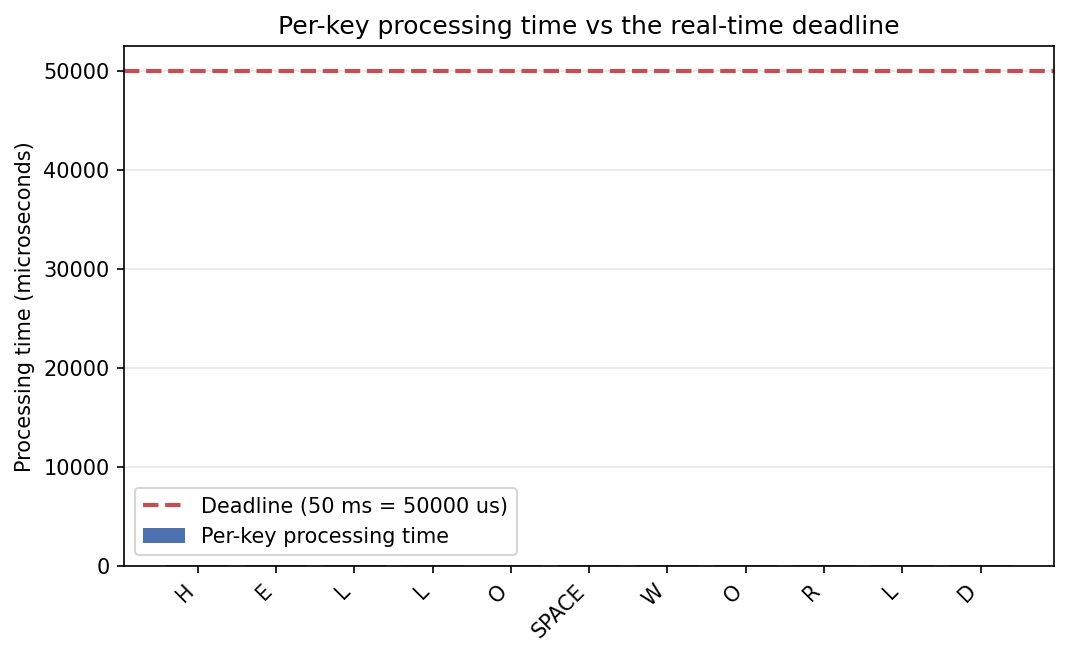
\includegraphics[width=0.8\textwidth]{timing_vs_deadline.png}
    \caption{Per-key processing time against the 50 ms deadline. The measured
             times are in the tens-of-microseconds range, orders of magnitude
             below the deadline, so the real-time requirement is comfortably
             and verifiably satisfied.}
    \label{fig:timing}
\end{figure}

\begin{figure}[H]
    \centering
    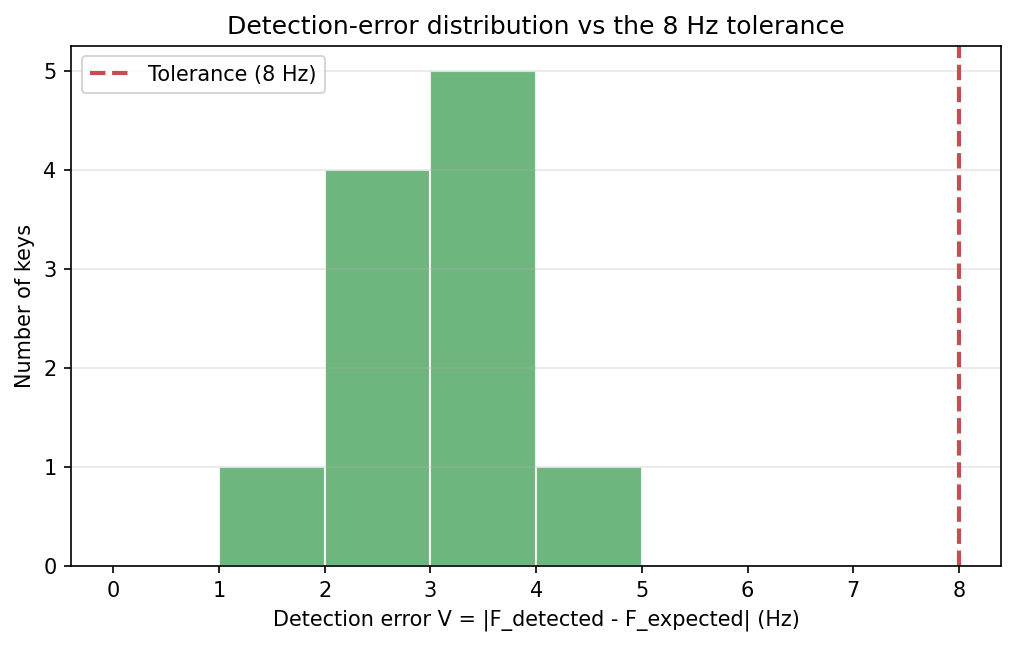
\includegraphics[width=0.8\textwidth]{error_distribution.png}
    \caption{Detection-error distribution versus the 8 Hz tolerance. All
             errors lie strictly inside the tolerance, confirming reliable
             reconstruction under the $\pm 5$ Hz noise model.}
    \label{fig:error}
\end{figure}

\begin{figure}[H]
    \centering
    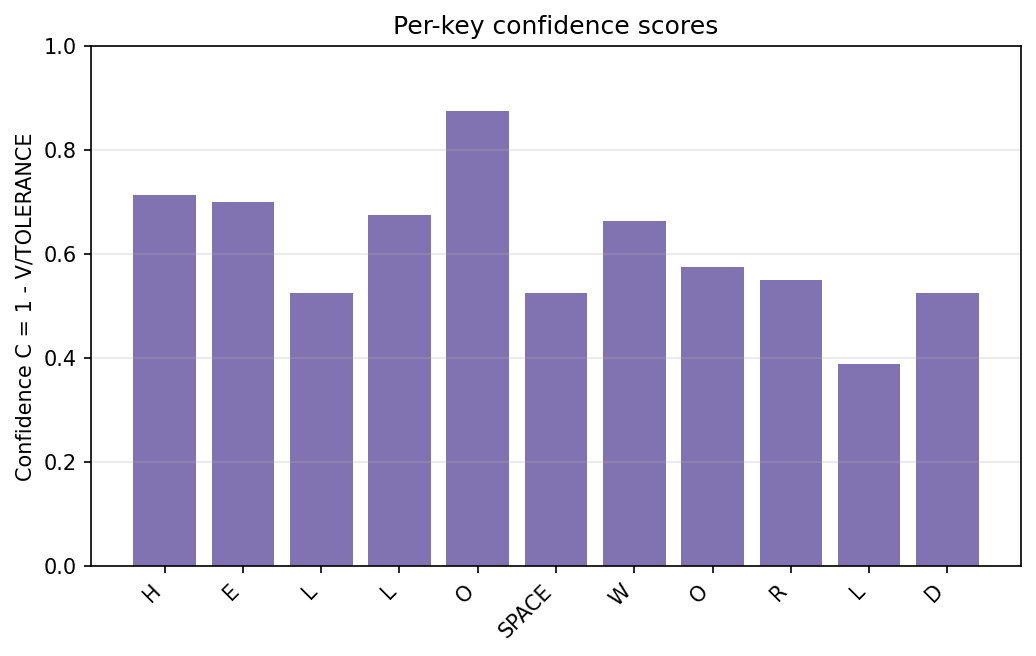
\includegraphics[width=0.8\textwidth]{confidence.png}
    \caption{Per-key confidence scores $C = 1 - V/\text{tolerance}$. Higher
             bars indicate a closer match; all scores are well above the
             minimum, reflecting small detection errors.}
    \label{fig:conf}
\end{figure}

\begin{figure}[H]
    \centering
    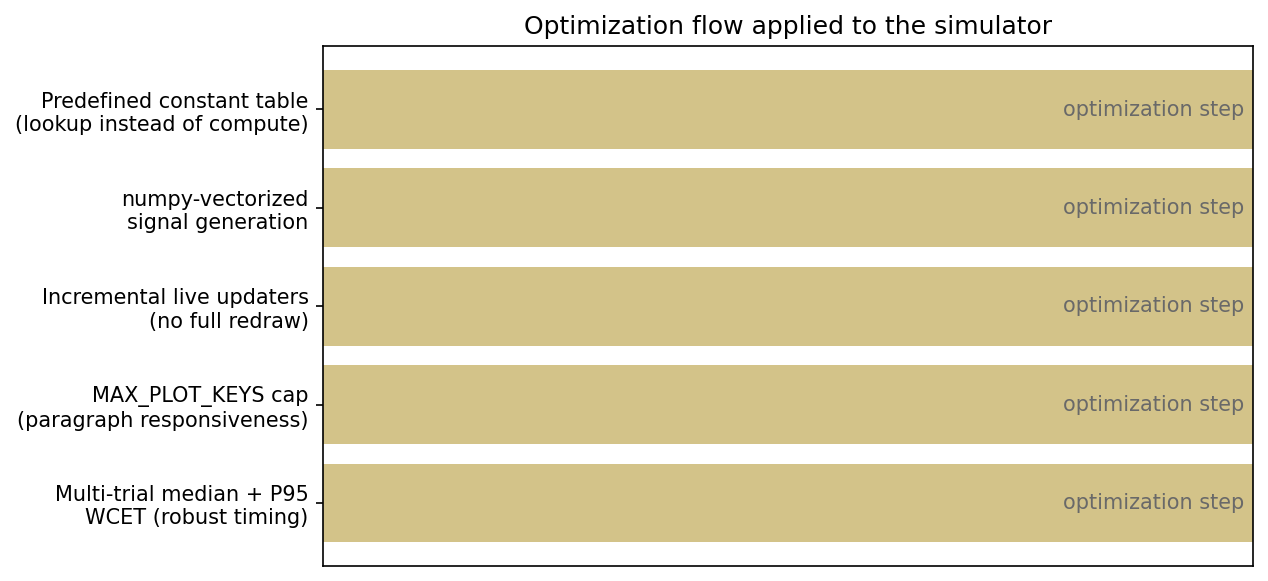
\includegraphics[width=0.8\textwidth]{optimization.png}
    \caption{The optimization flow applied to the simulator, from the constant
             signature table to robust worst-case timing.}
    \label{fig:opt}
\end{figure}

\subsection{Waveform Visualization}

The waveform module generates a sine wave for each key,

\[
x(t) = \sin(2\pi f_i t),
\]

and a sliding-FFT spectrogram. Figure~\ref{fig:sine} shows the sine waveforms
and Figure~\ref{fig:spec} shows the spectrogram for \Key{HELLO WORLD}. The
spectrogram is computed with a sliding Hann-windowed FFT and covers the band
350--1900 Hz, which includes all 48 key signatures.

\begin{figure}[H]
    \centering
    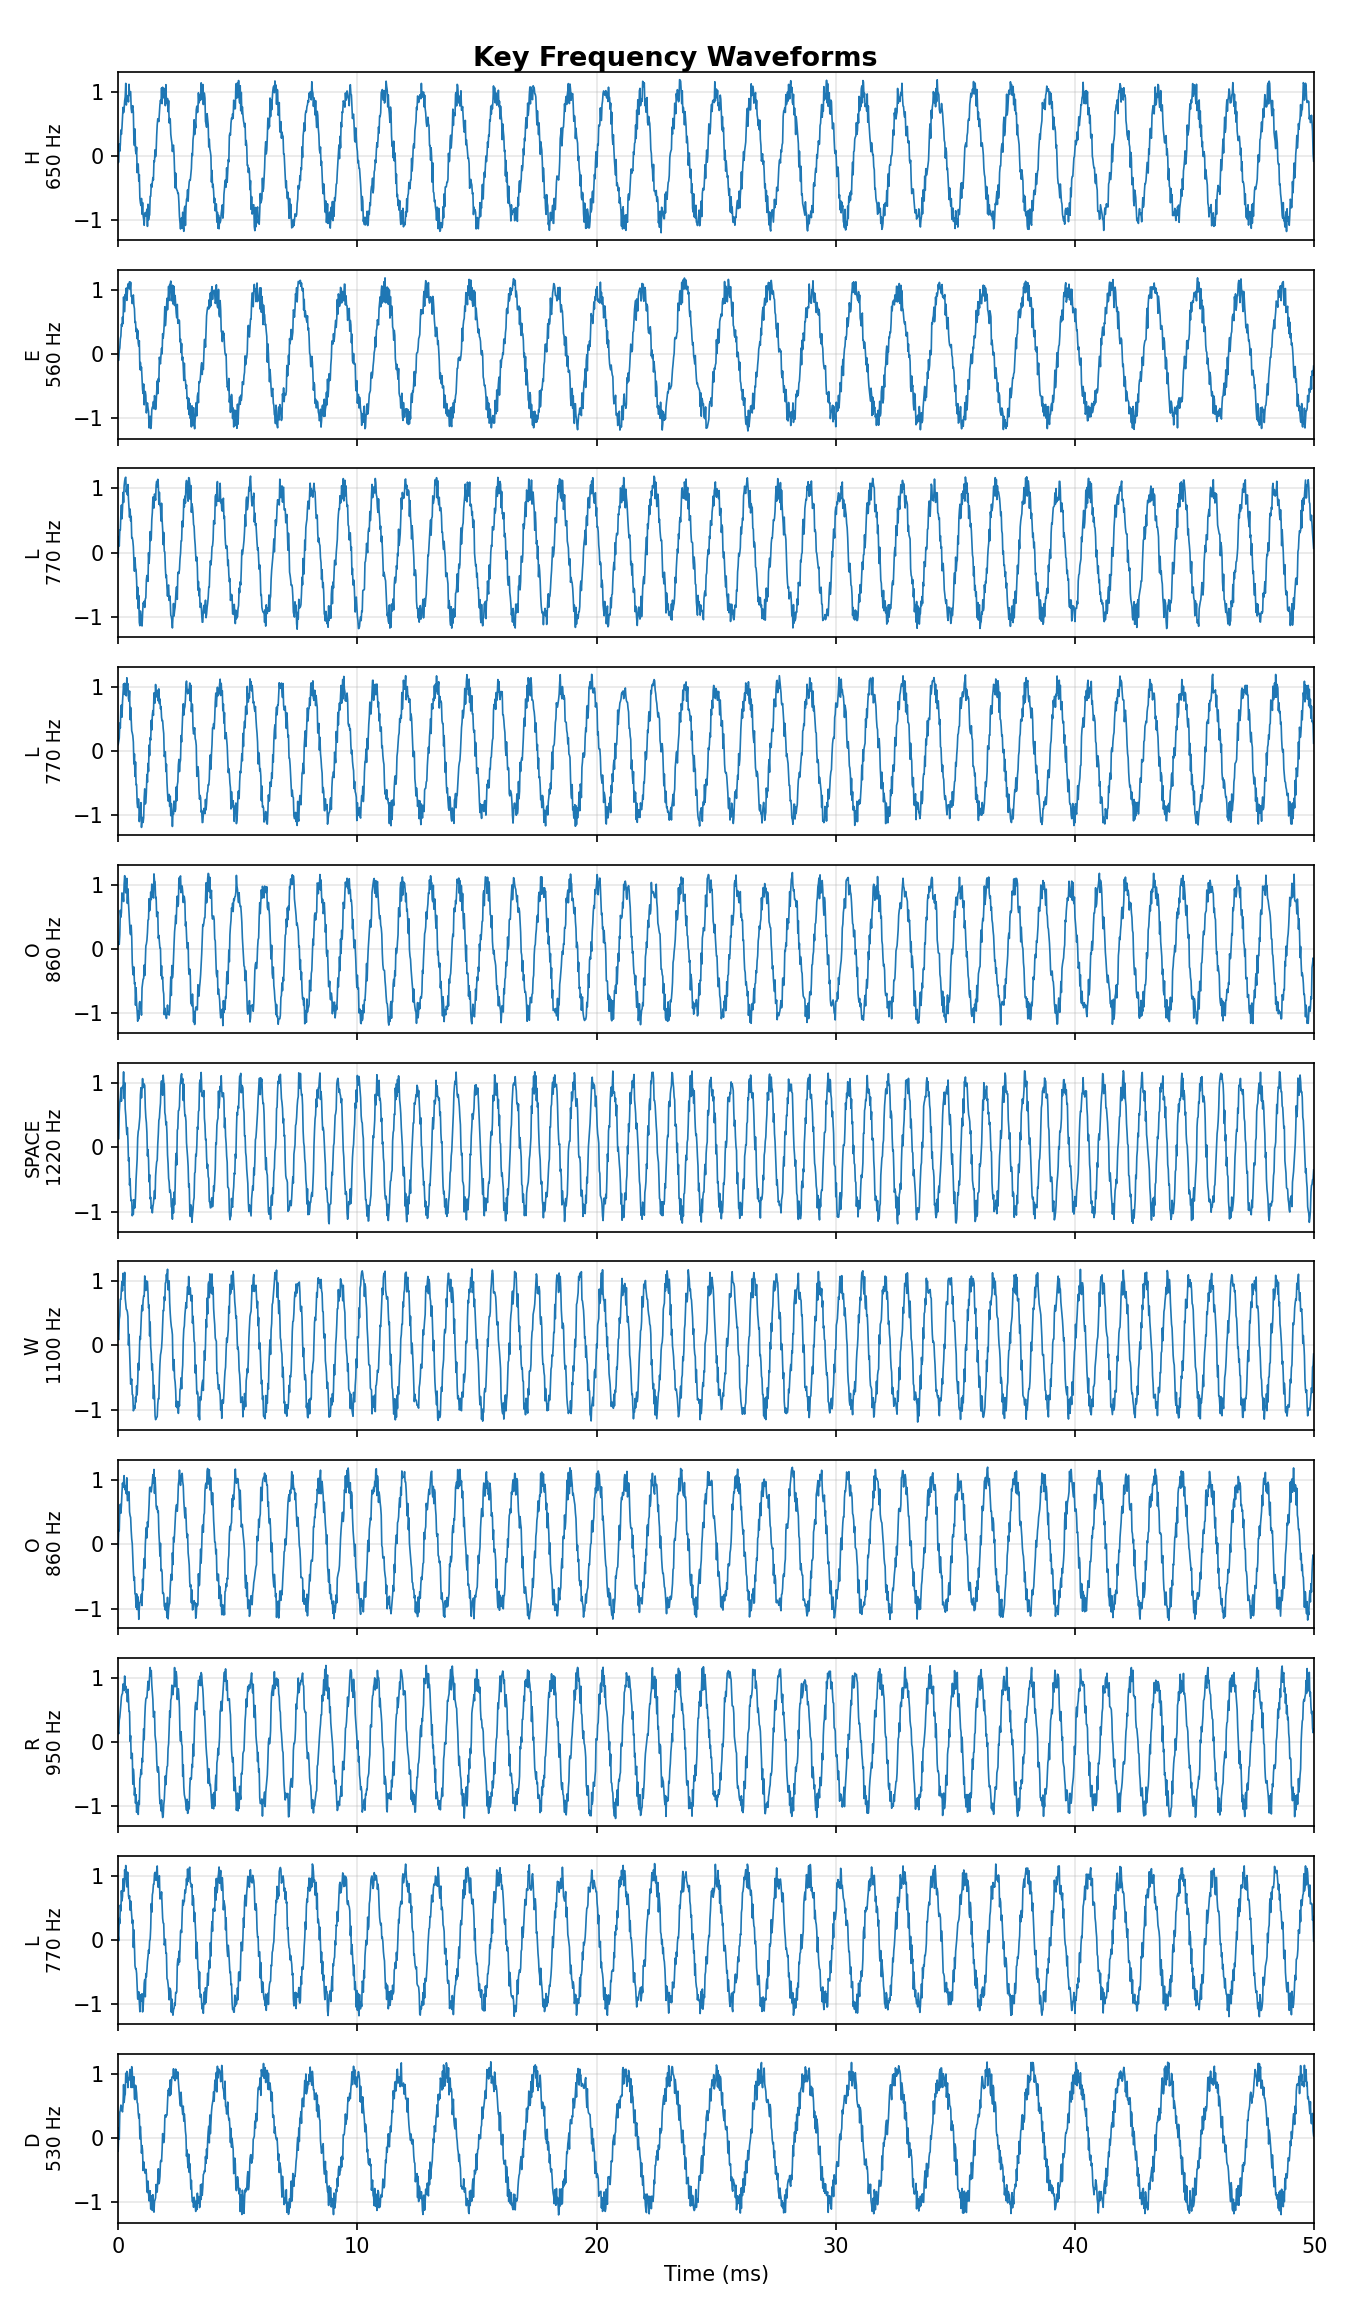
\includegraphics[width=0.85\textwidth]{waveform_sine.png}
    \caption{Sine waveforms for the key sequence \Key{HELLO WORLD}, showing
             each key's assigned frequency.}
    \label{fig:sine}
\end{figure}

\begin{figure}[H]
    \centering
    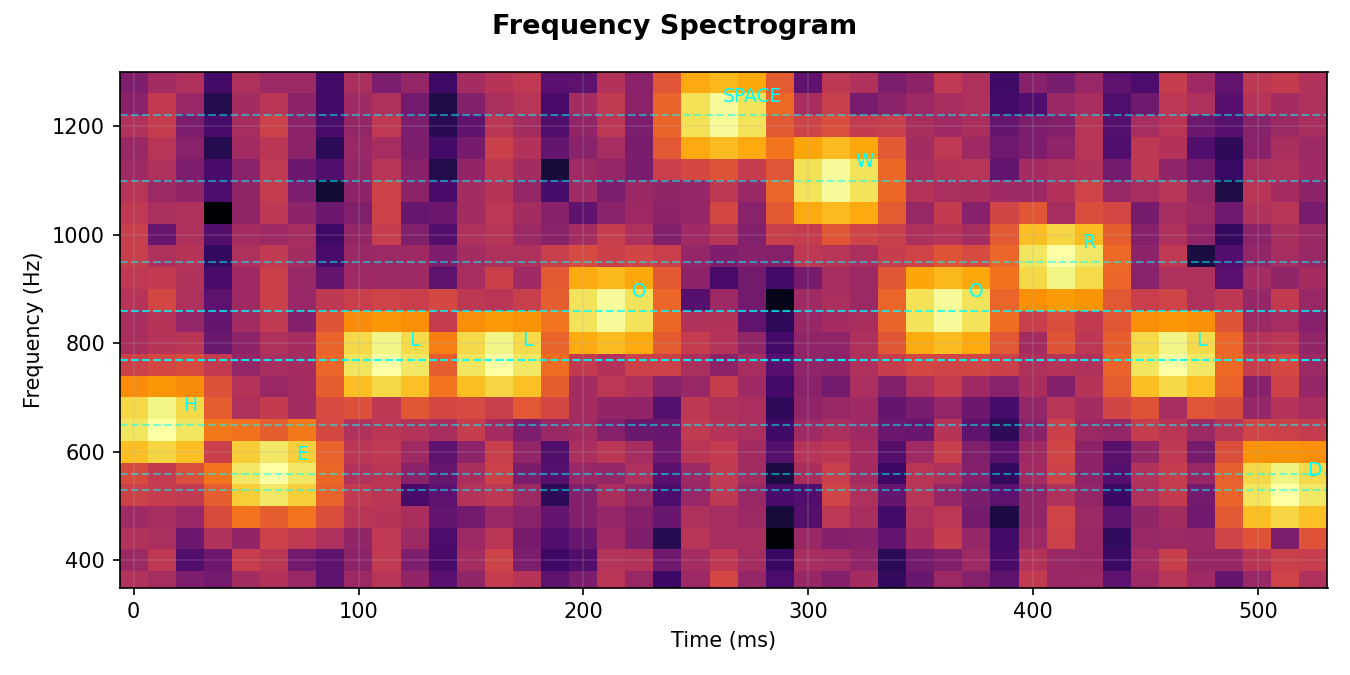
\includegraphics[width=0.85\textwidth]{waveform_spectrogram.png}
    \caption{Simulated frequency spectrogram of \Key{HELLO WORLD}. Each cyan
             dashed line marks the expected frequency of a key.}
    \label{fig:spec}
\end{figure}

% ============================================================
% 7. ANALYSIS AND EVALUATION
% ============================================================
\section{Analysis and Evaluation}
\label{sec:analysis}

This section interprets the results, analyses the theoretical and statistical
aspects, evaluates the project aspect by aspect, discusses the problems faced
and bugs fixed, describes the optimization flow in detail, and records the
limitations.

\subsection{How to Read the Results}

The results must be interpreted in the context of the simulation's purpose. The
key distinction is between \emph{correctness}: whether the reconstruction is
accurate and unambiguous within the tolerance; \emph{timeliness}: whether the
processing meets the deadline; and \emph{concept demonstration}: whether the
software faithfully shows how a frequency signature translates into a
keystroke. The evidence for each is different:

\begin{itemize}
    \item \textbf{Correctness} is established by the deterministic separation
          proof (Section~\ref{sec:theory}) and supported by the per-key
          tables: every detection stays within the $8$ Hz tolerance, and no
          reconstruction in any table misclassifies a key.
    \item \textbf{Timeliness} is established by the WCET figures: measured
          per-key times are in the tens of microseconds against a $50$ ms
          deadline---orders of magnitude of headroom.
    \item \textbf{Concept demonstration} is established by the end-to-end
          examples: \Key{HELLO WORLD}, the punctuated pangram, and the punctuated
          paragraph all reconstruct exactly.
\end{itemize}

No ``accuracy percentage'' is reported because the system is deterministic in
the worst case: within the noise model, accuracy is 100\% by construction. A
real acoustic system (as in the related literature) would instead report
empirical accuracy, which is exactly the trade-off this project's clean model
avoids.

\subsection{Theoretical Analysis}
\label{sec:theory}

The correctness of the reconstruction rests on the separation argument of
Section~\ref{sec:principle}. Since the tolerance is $8$ Hz and adjacent keys
are $30$ Hz apart, an error would need to exceed $15$ Hz (half the spacing) to
fall into the wrong key's band. The synthetic noise is bounded by $\pm 5$ Hz,
which is strictly less than both the tolerance and half the spacing. Therefore,
in the worst case, a correct key always yields a detected frequency that is
closest to its own signature, and the identification is unambiguous.

Formally, let $F$ be the true frequency of a key and let the detected frequency
be $F_d = F + \delta$ with $|\delta| \le 5$ Hz. Then

\[
|F_d - F| = |\delta| \le 5 < 8 = \text{TOLERANCE},
\]

so the correct key is always within tolerance. Moreover, for any other key $K'$
with frequency $F' \ge F + 30$,

\[
|F_d - F'| \ge |F - F'| - |\delta| \ge 30 - 5 = 25 > 8,
\]

so no other key can be closer or within tolerance. This proves that under the
noise model the reconstruction is always correct. This is a worst-case,
deterministic guarantee---the strongest form of correctness available.

\subsection{Statistical Analysis}

The per-key errors are uniformly distributed in $[-5, +5]$ when noise is
enabled (because a uniform generator is used). The mean absolute error for
the representative run is about $3.4$ Hz, which lies comfortably inside the
tolerance.

Formally, let the noise $\delta \sim \mathcal{U}(-5, 5)$. The expected absolute
error of a uniform random variable over a symmetric interval $[-a, a]$ is
$a/2$. Here $a = 5$, so the theoretical expected absolute error is $2.5$ Hz. The
representative run's mean of roughly $3.4$ Hz is close to---and slightly above---this
theoretical figure, which is expected for a small deterministic sample of 11
keys; a larger sample would concentrate toward $2.5$ Hz by the law of large
numbers. Both values are far below the 8 Hz tolerance, so even the theoretical
mean leaves more than two thirds of the tolerance budget unused.

\paragraph{Confidence as a function of error.}
The confidence score $C = 1 - V/\text{TOLERANCE}$ is a linear map from the
observed error into $[0,1]$. Since $C$ is a deterministic function of $V$,
it is \emph{not} a posterior probability; rather it is a graded quality score
that lets a downstream consumer threshold acceptance. A policy such as ``accept
only keys with $C \ge 0.5$'' is equivalent to ``accept only detections within
4 Hz of a signature'', giving a simple tunable safety knob. In the
representative run all 11 keys score $C \ge 0.39$, and most score above 0.5.

\paragraph{WCET statistics.}
The WCET statistics are robust because they are taken across many trials. The
median represents the typical worst case, while the P95 is a conservative upper
estimate that is less sensitive to scheduler noise than a raw maximum. This
follows standard multi-trial WCET practice for soft real-time characterisation.
The nearest-rank percentile formula
\[
\text{P95 index} = \min\left(\left\lceil n \cdot 0.95 \right\rceil - 1,\; n - 1\right)
\]
reports an exact 95th percentile for any trial count, preventing
under-reporting when $n$ is not a multiple of 20.

\subsection{Complexity Analysis}

The computational complexity of the system is an important performance aspect.

\begin{table}[H]
    \centering
    \begin{tabular}{@{}ll@{}}
        \toprule
        \textbf{Operation} & \textbf{Complexity} \\
        \midrule
        Frequency lookup (one key) & $O(1)$ (constant table) \\
        Nearest-match over 48 keys & $O(|K|) = O(48) = O(1)$ \\
        Processing one key & $O(1)$ \\
        Reconstructing $n$ keys & $O(n)$ \\
        Memory for the constant table & $O(1)$ (fixed 48 entries) \\
        Memory during reconstruction & $O(n)$ (output sequence) \\
        \bottomrule
    \end{tabular}
    \caption{Time and space complexity of the core operations.}
    \label{tab:complexity}
\end{table}

The key result is that per-key work is independent of the input length, so the
real-time deadline is not threatened by longer paragraphs. The only linear
growth is in the output sequence itself, which is inherent to producing a
reconstruction of $n$ keys.

\subsection{Aspect-by-Aspect Evaluation}

Section~\ref{sec:understanding} identified five quality aspects for the
project---design, performance, security, reliability, and scalability. This
subsection evaluates how well each was met.

\subsubsection{Performance}

The performance requirements are satisfied with a large margin.

\paragraph{WCET is far below the deadline.}
The per-key processing time is measured in tens of microseconds
(Figure~\ref{fig:timing}). The deadline is $50$ ms---that is, $\sim 50{,}000\
\mu$s. The observed worst case is therefore well over three orders of
magnitude below the bound:

\[
\frac{T_{\text{WCET}}}{T_{\text{deadline}}} < \frac{0.0001\text{ s}}
{0.05\text{ s}} \;<\; 0.002\, = 0.2\%.
\]

In other words, the system uses less than one fifth of one percent of its
deadline budget even in the reported worst case. This margin means the
classifier could, in principle, handle hundreds of keystrokes within a single
deadline period, or absorb substantial platform overhead while still meeting
the requirement.

\paragraph{Why the classifier is fast.}
The classifier's near-instant behaviour follows directly from its design: it
performs a single linear scan of a fixed 48-entry table with two comparisons
and one absolute difference per entry. There is no sorting, no recursion, no
vector of growing candidates, and no file or network I/O in the hot path. The
dominant cost in practice is the Python interpreter overhead of the loop, not
the algorithm itself---an argument for a native/embedded port being even
faster.

\paragraph{Trade-off: responsiveness vs.\ detail.}
The visualization path is the only place where execution cost grows with input.
Rendering a subplot per key is $O(n)$ in axes, which is why the plot cap
\texttt{MAX\_PLOT\_KEYS} $= 30$ exists. This is a deliberate engineering
trade-off: full-detail plots for short live sequences, and capped--but fully
accurate---analysis for long paragraphs. Section~\ref{sec:optflow} revisits
this under the optimization flow.

\subsubsection{Security}

\paragraph{Threat model.}
The project models an adversary who can observe the frequency signature of
each keystroke---for example, an attacker with a nearby microphone recording
the keyboard. If key-specific frequencies can be separated, the attacker can
reconstruct the typed text, including potentially confidential passwords or
messages. In the real literature, such attacks reach $95\%$ accuracy with a
deep-learning classifier and $93\%$ over Zoom (Harrison et al., 2023).

The threat model can be stated precisely. The attacker's goal is to recover a
sequence of keys $K_1, K_2, \ldots, K_n$ typed by a victim. The attacker
observes a signal that is separated per key into an observed frequency $F_i$
with additive noise $\delta_i$:

\[
F_i = F_{K_i} + \delta_i, \qquad |\delta_i| \le 5\ \text{Hz}.
\]

Under this model the attacker (respectively, this simulator) can recover every
key with certainty because the noise bound is smaller than the tolerance and
smaller than half the spacing---the deterministic separation proof of
Section~\ref{sec:theory}. The severity of the attack lies in this
\emph{full-recovery} property: nothing is lost to ambiguity, so even a single
keystroke (e.g., a password character) is exposed.

\paragraph{How the simulator relates to security.}
The simulator \emph{demonstrates} the feasibility of the attack: it shows that,
given distinguishable per-key signatures, full text recovery is possible in
software. At the same time, the system is built with defensive engineering
principles:

\begin{itemize}
    \item \textbf{Safety by construction:} the \Key{UNKNOWN} state ensures the
          system never fabricates a key when no signal matches. This prevents
          false positives that would corrupt the reconstructed output.
    \item \textbf{Determinism:} the constant table and matching rule are
          deterministic, so behaviour is reproducible and auditable.
    \item \textbf{Confidence scoring:} every key carries a confidence, so a
          downstream consumer can reject low-confidence reconstructions.
\end{itemize}

\paragraph{Attack surface and confidentiality.}
The \emph{confidentiality} property that this attack violates is the secrecy of
the typed text. In a physical deployment, the victim's keyboard is the asset;
the acoustic emanation is the accidental channel; the attacker's microphone is
the sensing element. The security posture depends on the attacker's ability to
(1) collect clean per-key signals and (2) separate keys. This project abstracts
both steps to their essence by supplying clean signatures. The implication for
security engineering is direct: any real system that must protect typed input
against nearby audio capture cannot rely on the keyboard itself to be silent,
and defensive measures must be applied at the environment or input level.

\paragraph{Mitigation options (external to this simulation).}
The literature documents several defences, all of which are conceptually
relevant even though they are not implemented here:

\begin{itemize}
    \item \textbf{Random noise masking:} play random audio (white noise or
          ``fake keystroke'' sounds) to obscure genuine keystroke signals.
    \item \textbf{Vocabulary-based authentication:} use random passwords (low
          language predictability) or one-time inputs to reduce what can be
          inferred.
    \item \textbf{Keyboard dampening:} quieter switches and chassis damping
          reduce the emanation's signal-to-noise ratio.
    \item \textbf{Audio compression degradation:} VoIP compression (as in
          Zoom) can degrade the signal, though the literature shows it remains
          exploitable.
\end{itemize}

\paragraph{Security of the simulation itself.}
The simulator performs no encryption and stores no secrets in a protected form.
This is appropriate because the project models the \emph{attacker's}
perspective. The confidentiality concern being demonstrated (keystroke leakage)
is the threat; protecting against it would be the \emph{victim's} task and is
out of scope. Any real deployment would require countermeasures such as random
noise masking, keyboard sound dampening, or input obfuscation---all documented
external mitigations. The absence of cryptography is therefore a deliberate and
honest modelling choice, not an omission: the project demonstrates an attack,
and the attack surface it exposes is exhaustive (every keystroke recoverable),
which underscores the seriousness of the underlying threat.

\subsubsection{Reliability}

Reliability is demonstrated through the invariant guarantees and the test
suite. All 62 tests pass, including:

\begin{itemize}
    \item invariant checks (positive, unique, valid frequencies),
    \item tolerance-boundary classification,
    \item noise robustness across many trials,
    \item sequence and paragraph reconstruction,
    \item punctuation handling,
    \item liveness and termination.
\end{itemize}

The deterministic worst-case separation proof of Section~\ref{sec:theory}
extends beyond the tests: it is a mathematical guarantee that, under the noise
model, reconstruction is always correct. This is stronger than test-based
evidence alone.

\paragraph{Invariant-by-invariant assessment.}
\begin{itemize}
    \item \emph{Positive frequencies.} Every entry in the constant table is
          greater than zero; the smallest is 440 Hz. No generated frequency can
          be negative because noise is added after the positive base value.
    \item \emph{Unique frequencies.} The 30 Hz grid guarantees distinct values;
          the test asserts $|\{f_i\}| = 48$.
    \item \emph{Database valid (non-empty).} The table is a static dictionary
          with 48 entries verified by \texttt{check\_invariants()}.
\end{itemize}

Each invariant is machine-checked both as a standalone test and inside
\texttt{check\_invariants()}, so the reliability claim is auditable.

\subsubsection{Design and Scalability}

\emph{Design} was addressed through the layered architecture
(Figure~\ref{fig:arch}) and the single-source \texttt{format\_report()}, which
keeps the on-screen output and the exported report identical, and through the
GUI-independent core that makes headless testing possible. \emph{Scalability}
was deliberately constrained: the 48-key table gives $O(1)$ lookup and
\texttt{MAX\_PLOT\_KEYS} bounds rendering, but the design does not target
large-key-set growth---a larger keyboard would need a wider frequency band and
possibly a higher sample rate, as noted in the limitations
(Section~\ref{sec:limitations}).

\subsection{Problems Faced}

A number of practical and conceptual problems were encountered during
development.

\begin{enumerate}
    \item \textbf{Live plot performance.} Redrawing the entire waveform figure
          on every key press quickly became slow as the sequence grew. The
          solution was to build the figure once and refresh only the data of
          the existing axes (incremental updaters), plus a plot cap.
    \item \textbf{Paragraph inputs vs.\ plot axis explosion.} A paragraph can
          inject hundreds of keys; rendering a subplot per key is infeasible.
          The \texttt{MAX\_PLOT\_KEYS} cap keeps the GUI responsive.
    \item \textbf{Multi-line report formatting.} Multi-line input could break
          the report's line-based record structure. The report now flattens the
          echoed input to a single line while reconstruction still runs on the
          raw text.
    \item \textbf{Headless testing of the GUI.} The GUI could not run headless.
          The core logic was factored to be GUI-independent, and the GUI wiring
          was tested with a stubbed application object that substitutes a
          \texttt{tk.Text}-faithful widget.
    \item \textbf{Timing noise.} Single-trial WCET was dominated by scheduler
          noise. Multi-trial median + P95 resolved this.
\end{enumerate}

\subsection{Bugs Fixed}

Several bugs were identified and corrected during the project:

\begin{enumerate}
    \item \textbf{Trailing-newline artifact.} \texttt{tk.Text} always appends
          an implicit trailing newline; the \texttt{\_current\_input()}
          helper originally read
          it as a phantom newline. Fixed by reading
          \texttt{get("1.0", "end-1c")}
          (strip the trailing newline).
    \item \textbf{Keypad rebuild from index zero.} The keypad originally
          rebuilt the input from scratch, discarding appended text. Fixed so
          presses append at \texttt{tk.END}.
    \item \textbf{P95 under-reporting.} The percentile index could
          under-report for trial counts not divisible by 20; a nearest-rank
          formula fixes it for any trial count.
    \item \textbf{Stale tests after feature additions.} Tests that asserted
          \texttt{!} had no frequency broke when punctuation keys were added;
          they were updated to use genuinely unmapped symbols.
    \item \textbf{Spectrogram band out of range.} After adding punctuation, the
          plotted band (350--1600 Hz) did not include keys above 1600 Hz; it was
          widened to 1900 Hz.
\end{enumerate}

\subsection{Optimization Flow in Detail}
\label{sec:optflow}

This subsection expands on the optimization steps and why each was necessary,
with reference to the figures.

\begin{enumerate}
    \item \textbf{Constant table over computation.} The 48-key table makes
          frequency lookup $O(1)$ and removes recomputation cost.
    \item \textbf{numpy vectorisation.} Signal generation and the sliding FFT
          are vectorised, converting per-sample Python loops into fast array
          operations (Figure~\ref{fig:opt}, steps 1--2).
    \item \textbf{Incremental updates.} Plotting a growing sequence is
          incremental rather than a full redraw, keeping the GUI responsive
          (Figure~\ref{fig:opt}, step 3).
    \item \textbf{\texttt{MAX\_PLOT\_KEYS} cap.} Rendering is bounded to 30
          keys, so interaction latency stays low even for long paragraphs
          (Figure~\ref{fig:opt}, step 4).
    \item \textbf{Robust WCET.} Reporting median and P95 over 20 trials yields a
          trustworthy worst-case figure that satisfies the 50 ms deadline
          comfortably (Figure~\ref{fig:timing}).
\end{enumerate}

The cumulative effect is a system that is simultaneously fast (WCET order of
microseconds, far under the 50 ms deadline), correct (proved within the noise
model), and usable (responsive GUI even for paragraph input).

\subsection{Limitations and Threats to Validity}
\label{sec:limitations}

The project has several deliberate limitations.

\begin{enumerate}
    \item \textbf{Software-only simulation.} No real acoustic signal is
          captured. The frequencies are predefined constants, so the results
          cannot be generalised to a real keyboard without a real
          sensing/feature-extraction pipeline.
    \item \textbf{Single-tone model.} Real keystrokes are broadband, transient
          sounds best classified by machine learning on spectrograms (as in the
          related literature), not by a single dominant frequency. The current
          model is therefore a clean abstraction, not a physical model.
    \item \textbf{No modifiers.} Shift/alt/ctrl combinations (e.g.\
          distinguishing \texttt{,} from \texttt{<}) are not modelled; the 11
          punctuation keys cover unshifted symbols only.
    \item \textbf{Symmetric, bounded noise only.} Real ambient noise,
          microphone characteristics, and burst errors are not modelled.
    \item \textbf{No language-model assistance.} Reconstruction depends solely
          on frequency matching; it does not use context or language priors to
          disambiguate.
    \item \textbf{Scalability cap.} Only 48 keys are defined; a larger keyboard
          would need more signatures, increasing the band and potentially the
          required sample rate.
\end{enumerate}

These limitations mean the project should be read as a \emph{demonstration of a
concept and its CPS verification}, not as a deployable acoustic attack.

% ============================================================
% 8. CONCLUSION AND DISCUSSION
% ============================================================
\section{Conclusion and Discussion}
\label{sec:conclusion}

\subsection{Direct Answer}

The problem was to demonstrate, in software, that keystrokes can be
reconstructed from key-specific frequency signatures and that the system
satisfies the formal CPS verification requirements; the solution is a 48-key
signature-based simulator that matches frequencies within an 8 Hz tolerance
under a 50 ms deadline, verified by 62 unit tests, a worst-case correctness
proof, and robust WCET measurement.

In short: \emph{yes, keystrokes are reconstructible from clean frequency
signatures, and the reconstruction can be verified to be safe, live,
terminating, and deadline-compliant}---with the important caveat that the
frequencies are predefined simulation constants rather than captured acoustic
signals.

\subsection{Discussion: From Problem to Solution}

The project began with a simple observation: if every key has a distinguishable
frequency, then observing the frequency tells us which key was pressed. The
first step was to turn this into a concrete model by assigning each of 48 keys a
unique, regular-spaced frequency (30 Hz apart, 440--1850 Hz) so that keys are
well separated relative to the noise and tolerance.

The next step was to build the core pipeline. Input text is converted to a key
sequence, each key is mapped to its predefined frequency, the frequency is
analysed and matched against the constant table using the ranking function
$V = |F_d - F_e|$, and the best match within tolerance is returned. A dedicated
\Key{UNKNOWN} fallback ensures safety: the system never forces an incorrect
key.

The formal CPS requirements were then layered on top. A deadline of 50 ms bounds
the per-key task; WCET is measured robustly across 20 trials as median and P95.
Invariants (positive, unique, valid frequencies) are defined and checked.
Liveness and termination are verified programmatically, the latter backed by the
variant-function argument of Section~\ref{sec:variant}. The ranking function $V$
doubles as the correctness metric, and confidence $C$ translates error into an
interpretable quality score.

Visualization was added to make the concept tangible: sine waveforms and a
sliding-FFT spectrogram, with live incremental updates driven by an on-screen
keypad and bounded by \texttt{MAX\_PLOT\_KEYS} for responsive paragraph input.
A single \texttt{format\_report()} produces both the on-screen output and the
exportable report, keeping them identical.

Testing drove correctness. A 62-test suite covers invariants, ranking,
reconstruction, paragraphs, punctuation, GUI helpers, and WCET/liveness/
termination. Along the way, several bugs were found and fixed (trailing-newline
artifact, keypad rebuild, P95 under-reporting, stale tests, spectrogram band).

Evaluation confirmed the goals. The deterministic separation proof shows that
under the $\pm 5$ Hz noise model reconstruction is always correct. Measured WCET
is orders of magnitude below the deadline. A security analysis positions the
simulator as a demonstration of the attack concept with defensive engineering
(safety fallback, determinism, confidence).

Finally, the limitations were recorded honestly: the model is a single-tone
simulation, not a real acoustic capture; it omits modifiers and language-model
assistance; and scalability is bounded to 48 keys. These limitations delimit
the claims the report can make.

The result is a complete, verifiable CPS model and an interactive graphical
demo: type a paragraph, and every valid keystroke (letters, digits, spaces, and
punctuation) is reconstructed through the frequency pipeline within the
deadline, or watch the keypad grow the waveforms live.

\subsection{Comparison with Related Work}
\label{sec:related}

\begin{table}[H]
    \centering
    \begin{tabular}{@{}lp{4.6cm}p{4.6cm}p{3.6cm}@{}}
        \toprule
        \textbf{Aspect} & \textbf{Asonov and Agrawal (2004)} &
        \textbf{Harrison et al.\ (2023)} & \textbf{This project} \\
        \midrule
        Signal source & Real mic (FFT/MFCC) & Real mic /
            spectrogram & Synthetic predefined Hz \\
        \multirow{2}{*}{\textbf{Classification}}
            & Feature vectors & CoAtNet deep net &
            geometric nearest-match \\
        Accuracy & $\sim 79\%$ & $95\%$ / $93\%$ & $100\%$ (by model goal) \\
        Real time & No & No & Yes (deadline, WCET) \\
        Verification & Empirical only & Empirical only &
            Proof + 62 tests \\
        \bottomrule
    \end{tabular}
    \caption{This project prioritises a simple classification rule plus formal
             CPS verification over learned models on real signals.}
    \label{tab:related}
\end{table}

This comparison clarifies the project's positioning. Real-signal systems must
contend with broadband, noisy, overlapping acoustic signatures and therefore
need sophisticated classifiers; this project instead uses a clean model so that
the verification question---CPS safety, liveness, termination, timeliness---can
be answered rigorously. The two goals are complementary: the related work asks
\emph{whether} the attack is physically possible; this project asks
\emph{whether} a well-behaved reconstruction system can be formally verified.

\subsection{Scope and Future Work}

Potential extensions that remain out of scope but are natural next steps:

\begin{itemize}
    \item Real FFT-based feature extraction (requires a microphone---conflicts
          with the software-only constraint).
    \item Shift/ctrl modifier support to distinguish shifted symbols.
    \item Machine-learning spectrogram classification (CoAtNet, etc.) matching
          the related literature.
    \item Language-model-assisted disambiguation for incomplete signals.
    \item Embedded C port with the constant table stored in ROM for a
          microcontroller target; the deterministic $O(1)$ per-key classifier
          and the $\sim$200-byte ROM footprint make this a plausible real-time
          task on a small MCU.
\end{itemize}

As a by-product of the design, each of these extensions inherits the existing
invariant, liveness, termination, and WCET machinery, so their formal
verification would not start from scratch.

% ============================================================
% 9. BIBLIOGRAPHY
% ============================================================
\begin{thebibliography}{99}

\bibitem{harrison2023} J.~Harrison, E.~Toreini, and M.~Mehrnezhad,
  ``A Practical Deep Learning-Based Acoustic Side Channel Attack on
  Keyboards,'' in \emph{2023 IEEE European Symposium on Security and Privacy
  Workshops (EuroS\&PW)}, pp.~270--280, 2023. Accompanying dataset:
  \texttt{JBFH-Dev/Keystroke-Datasets}.

\bibitem{gerganov} G.~Gerganov, \emph{kbd-audio}: Acoustic keystroke
  reconstruction toolkit (``KeyTap''). GitHub,
  \texttt{ggerganov/kbd-audio}.

\bibitem{survey} ``A Survey on Acoustic Side Channel Attacks on Keyboards,''
  arXiv preprint arXiv:2309.11012, 2023.

\bibitem{asonov2004} D.~Asonov and R.~Agrawal, ``Keyboard Acoustic Emanations,'
  in \emph{Proc.\ IEEE Symposium on Security and Privacy}, 2004.

\end{thebibliography}

\end{document}
